\documentclass[]{beamer}   	%standardeinstellung
\usepackage{amsmath}				%damit du formeln eingeben kannst
\usepackage[parfill]{parskip}    			% neuer absatz durch leere zeile
\usepackage{graphicx}				% bilder einfügen
\usepackage{hyperref}				%damit man links erstellen kann
\usepackage{float}					%intelligentes anpassen von bildern, damit es keine lücken im text gibt
\graphicspath{ {figures/} }				%automatisches erstellen von "List of Figures"
\usepackage[font=small,labelfont=bf]{caption} %formatierung der bildunterschrift
 \usepackage{geometry}				%Seitenlayout
 \usepackage{tikz}


\usepackage{ragged2e}
\usepackage[export]{adjustbox}
\usepackage{dsfont}
\usepackage{amssymb}
\usepackage{caption}
\usepackage{natbib}
\usepackage[utf8]{inputenc}
\usepackage{amsmath}
\usepackage{amsfonts}
\usepackage{amssymb}
\usepackage{wrapfig}
\usepackage{subcaption}
\usepackage{pdflscape}
\usepackage{filecontents,url}
\usepackage{soul}
\usepackage[space]{grffile}
\usepackage[UKenglish]{isodate}
\newcommand{\mysubcaption}[1]{
\justify
\begin{spacing}{0.7}
\textit{\footnotesize #1}
\end{spacing}}

\title{Spatial Inefficiencies in Africa's Trade Network}
\author{Tilman Graff}
\institute{University of Oxford}
\date{\today}

\begin{document}

\begin{frame}
  \titlepage
\end{frame}

\begin{frame}
  \frametitle{Motivation}
  \begin{figure}
    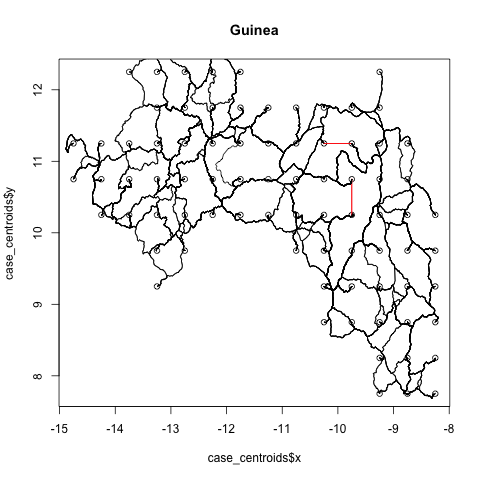
\includegraphics[width=0.6\textwidth, trim={1cm 1cm 0cm 2cm},clip]{/Users/Tilmanski/Documents/UNI/MPhil/Second Year/Thesis_Git/Build/output/Road_Networks/network_Guinea.png}
    \caption{Road Network Guinea}

  \end{figure}
\end{frame}

\begin{frame}
  \frametitle{Motivation}
\begin{figure}
    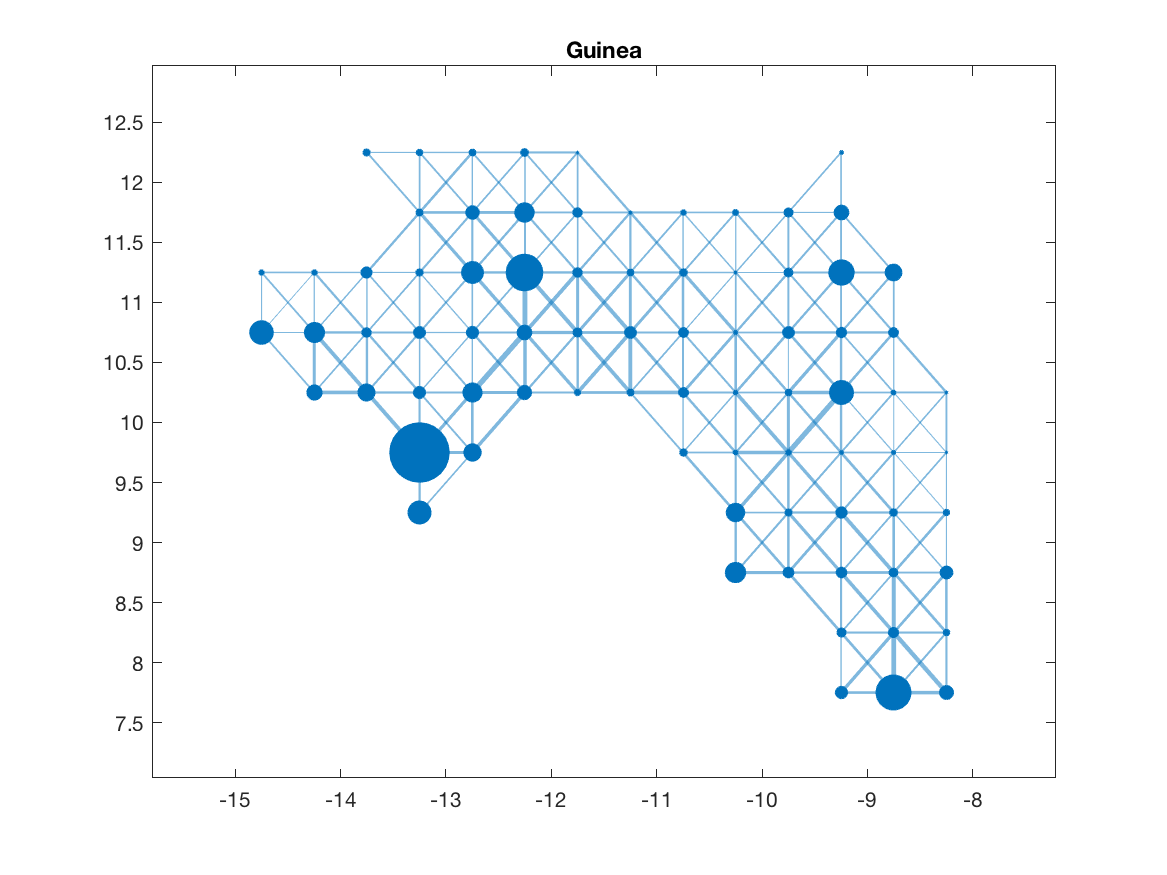
\includegraphics[width=0.6\textwidth, trim={2cm 1cm 1.5cm 0cm},clip]{/Users/Tilmanski/Documents/UNI/MPhil/Second Year/Thesis_Git/Build/output/Matlab_graphs/Nicer_graphs/Guinea_stat.png}
    \caption{Road Network Guinea}

  \end{figure}
\end{frame}

\begin{frame}
  \frametitle{Motivation}
\begin{figure}
    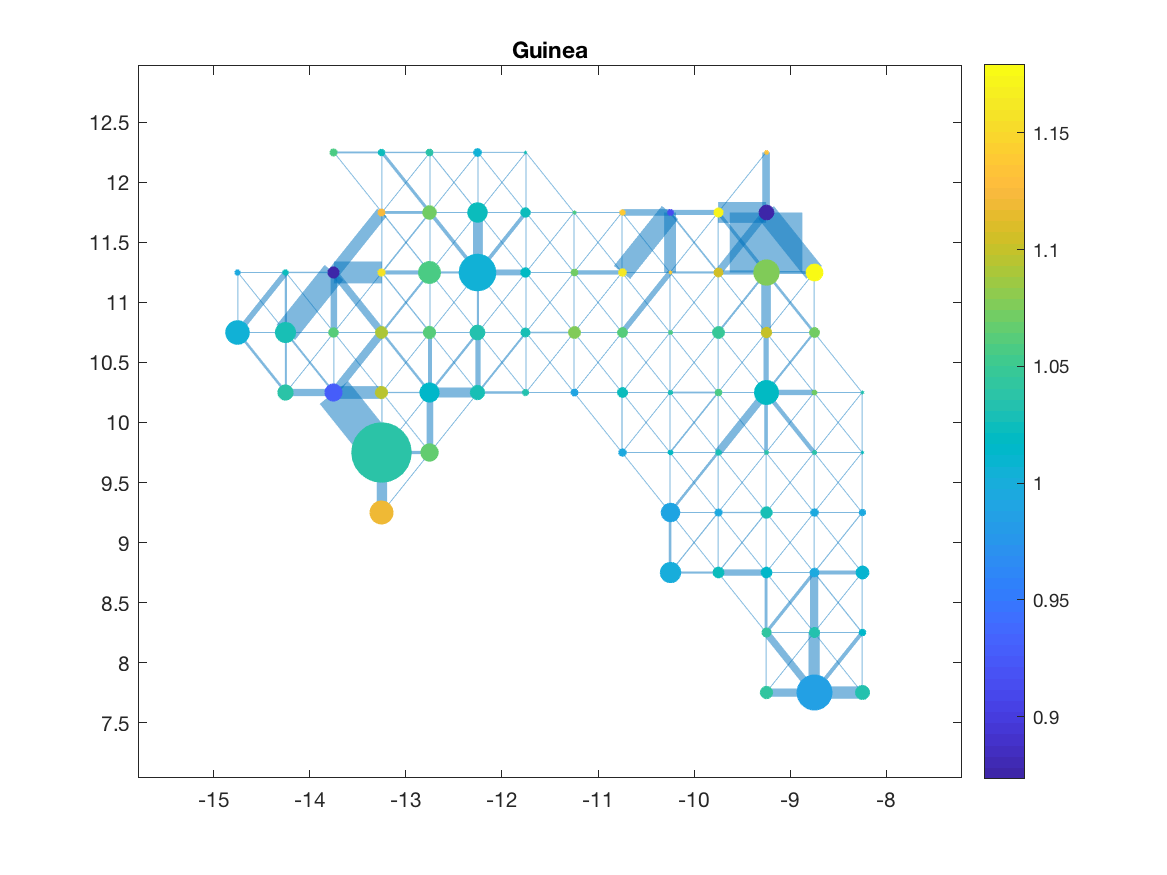
\includegraphics[width=0.6\textwidth, trim={2cm 1cm 1.5cm 0cm},clip]{/Users/Tilmanski/Documents/UNI/MPhil/Second Year/Thesis_Git/Build/output/Matlab_graphs/Nicer_graphs/Guinea_opt.png}
    \caption{Optimal Road Network Guinea}

  \end{figure}
\end{frame}

\begin{frame}
  \frametitle{Motivation}
  \begin{itemize}
    \item Are African roads where they should be?
    \item Which country has the most efficient trade network?
    \item Why do some regions have \emph{too} many roads?
  \end{itemize}
\end{frame}

% \setbeamercovered{transparent}
% \begin{frame}
%   \frametitle{Motivation}
%   \centering
%   \onslide<1->{Individual transport policies \\
%   $\Longleftrightarrow$} \\
%   \onslide<2->{Overall network efficiency}
% \end{frame}


\begin{frame}
  \frametitle{Steps}
  \setbeamercolor{normal text}{fg=gray,bg=}
\setbeamercolor{alerted text}{fg=black,bg=}
\usebeamercolor{alerted text}
  \begin{enumerate}
    \item Network representation for all African countries
    \begin{itemize}
      \item Nodes
      \item Edges
    \end{itemize}
    \item Employ in simple trade model
    \item Reshuffle roads to get optimal network
    \item Analyse patterns of reshuffling
  \end{enumerate}
\end{frame}

\begin{frame}
  \frametitle{Steps}
  \setbeamercolor{normal text}{fg=gray,bg=}
\setbeamercolor{alerted text}{fg=black,bg=}
\usebeamercolor{normal text}
  \begin{enumerate}
    \item \alert{Network representation for all African countries}
    \begin{itemize}
      \item \alert{Nodes}
      \item Edges
    \end{itemize}
    \item Employ in simple trade model
    \item Reshuffle roads to get optimal network
    \item Analyse patterns of reshuffling
  \end{enumerate}
\end{frame}

\begin{frame}
  \frametitle{Network Nodes}
  \begin{figure}
    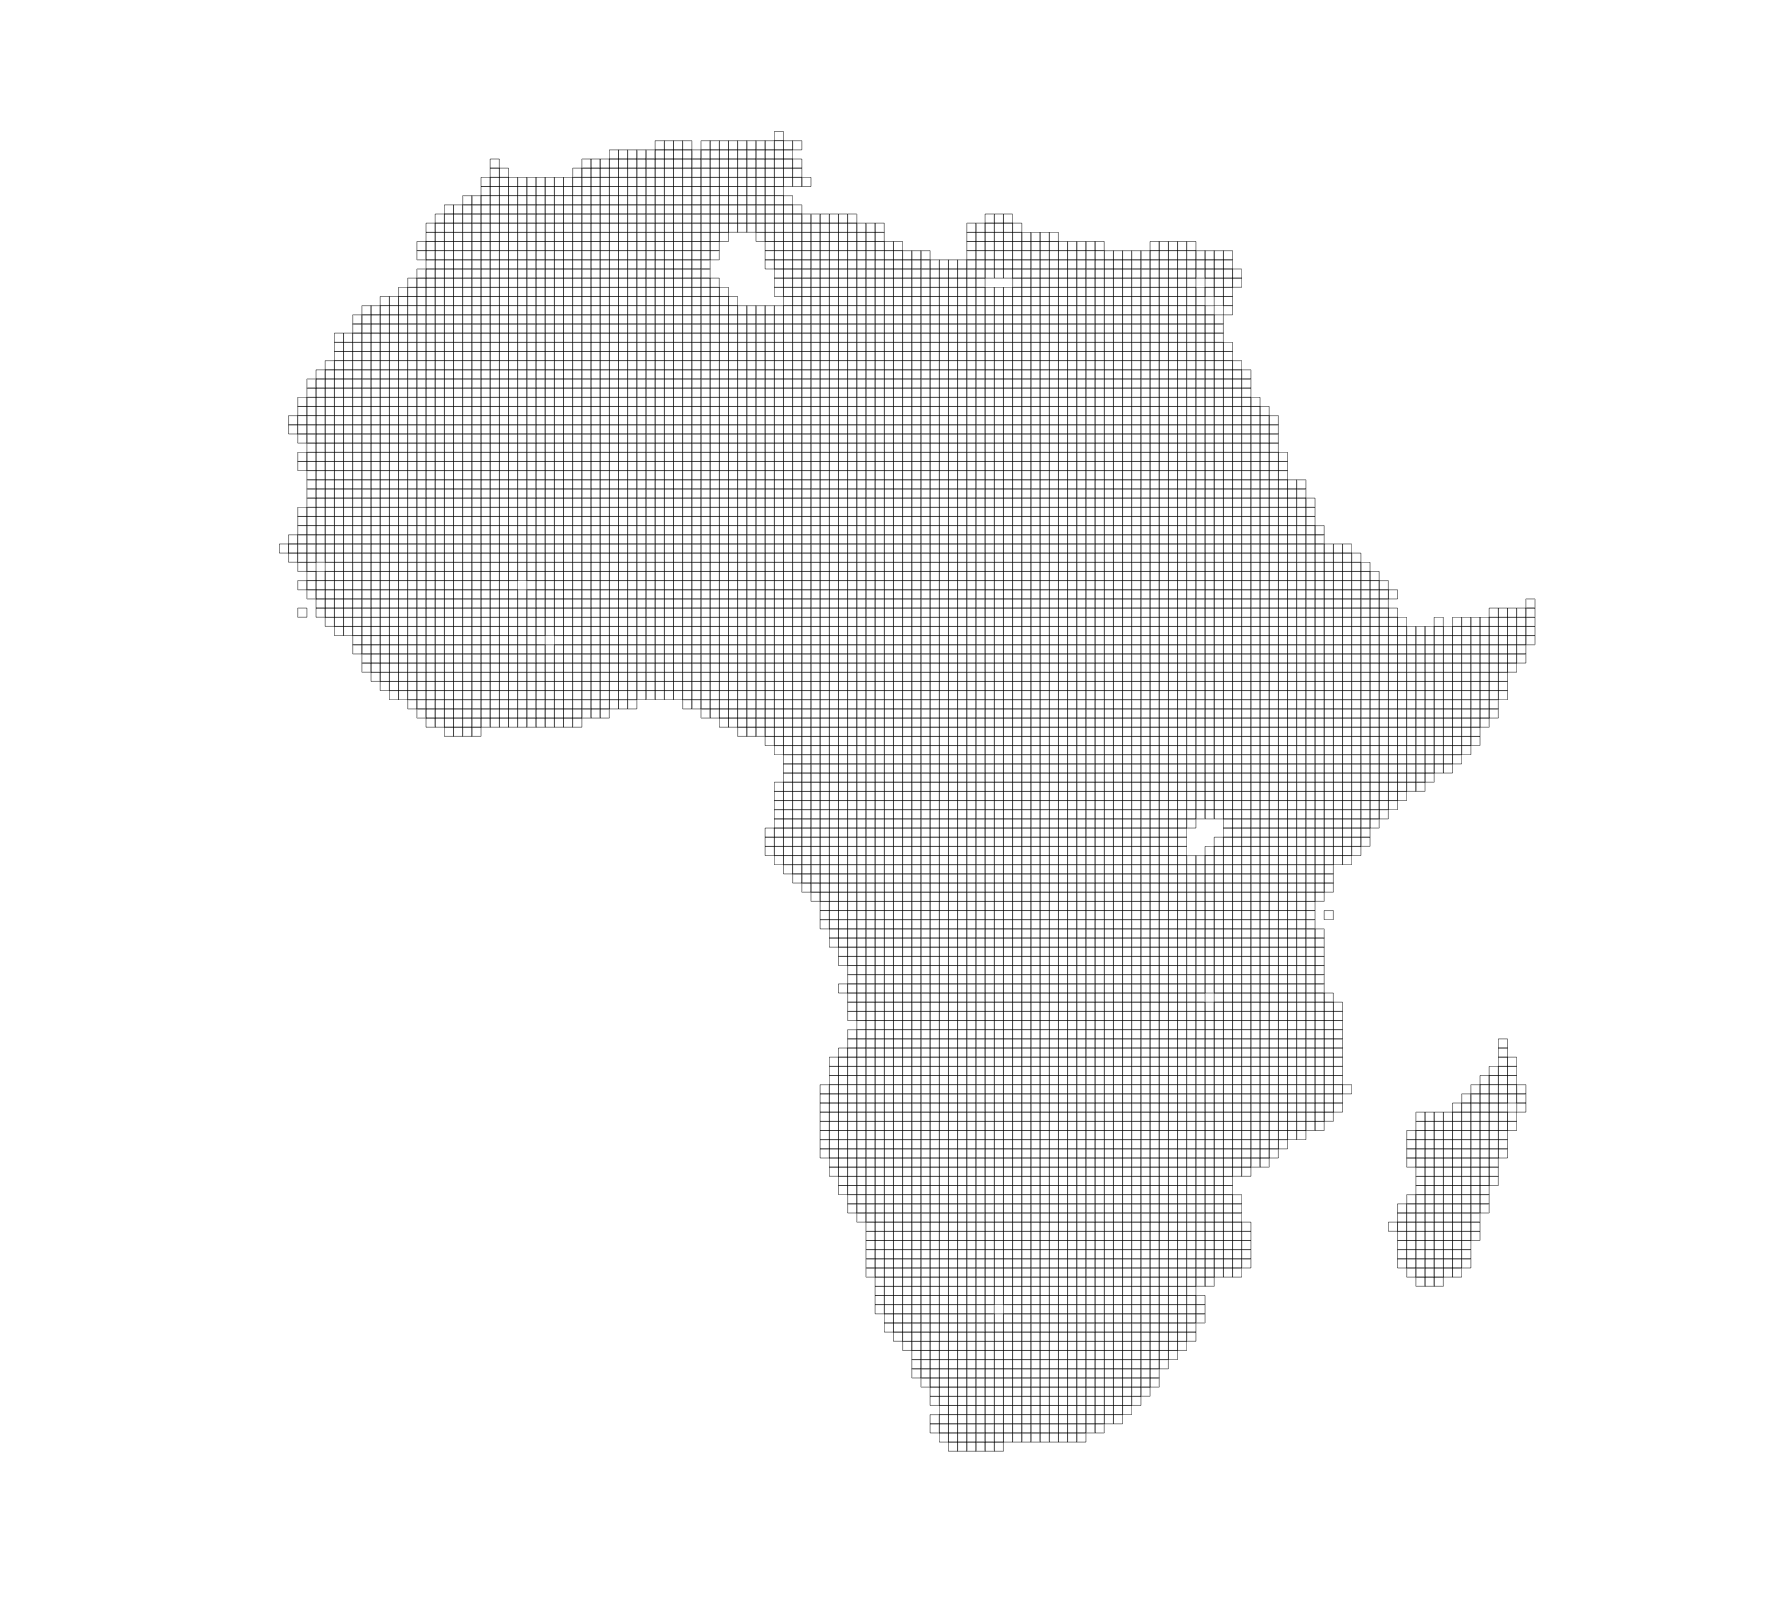
\includegraphics[width=0.85\textwidth, trim={1cm 4cm 0cm 2cm},clip]{/Users/Tilmanski/Documents/UNI/MPhil/Second Year/Thesis_Git/Write/Present/Images/African_grid.png}
    \caption{10,167 grid cells (0.5 x 0.5 degrees)}
  \end{figure}
\end{frame}

\begin{frame}
  \frametitle{Network Nodes}
  \begin{columns}
    \column{0.4\textwidth}
      \begin{itemize}
        \item Population
        \item Output (night lights)
        \item Geography
      \end{itemize}
    \column{0.6\textwidth}
  \begin{figure}
    \centering
    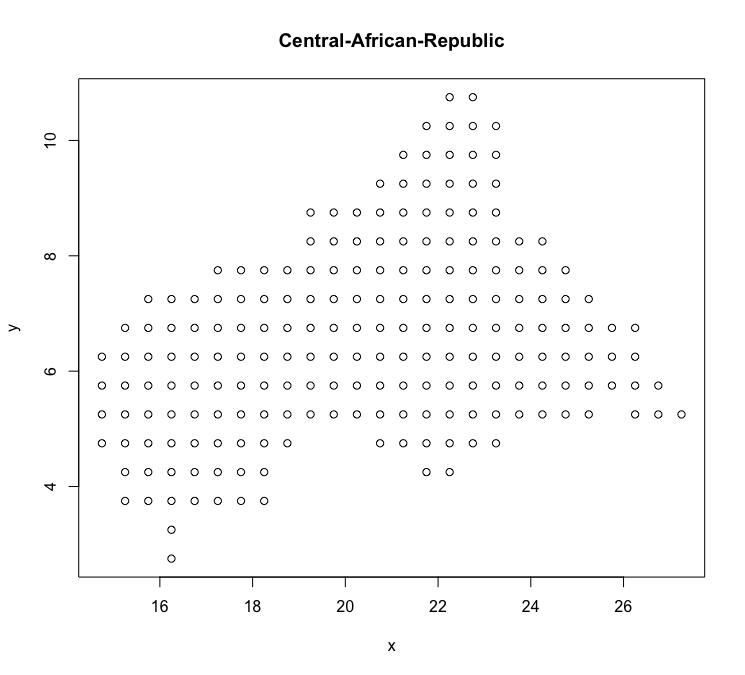
\includegraphics[width=\textwidth, trim={1cm 1.5cm 1cm 1cm},clip]{/Users/Tilmanski/Documents/UNI/MPhil/Second Year/Thesis_Git/Write/Present/Images/CAE_nodes.png}
  \end{figure}
  \end{columns}
\end{frame}

\begin{frame}
  \frametitle{Network Edges}
  \begin{columns}
    \column{0.4\textwidth}
      \begin{itemize}
        \item Average Speed
        \item Distance
        \item Topography
      \end{itemize}
    \column{0.7\textwidth}
  \begin{figure}
    \centering
    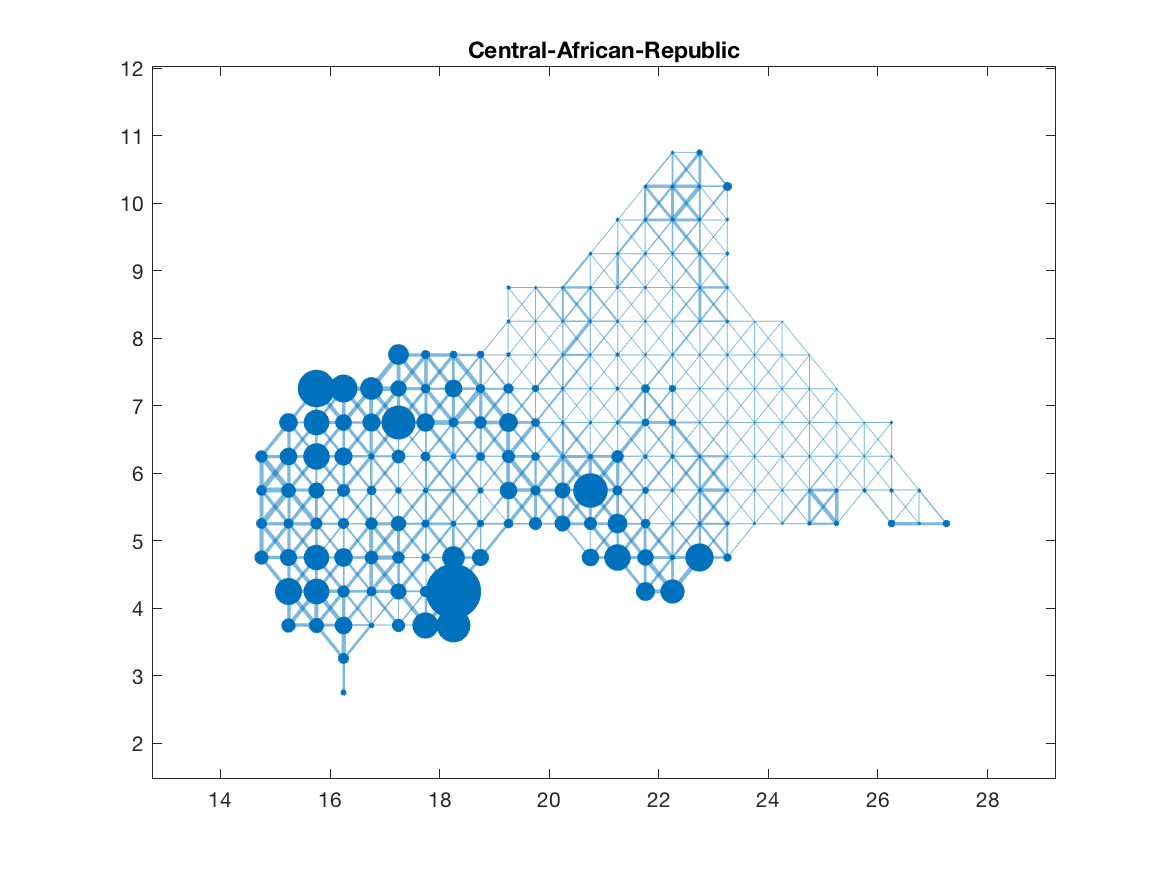
\includegraphics[width=\textwidth, trim={2cm 1cm 1.5cm 0cm},clip]{/Users/Tilmanski/Documents/UNI/MPhil/Second Year/Thesis_Git/Build/output/Matlab_graphs/Nicer_graphs/Central-African-Republic_stat.png}
  \end{figure}
  \end{columns}
\end{frame}

\begin{frame}
  \frametitle{Steps}
  \setbeamercolor{normal text}{fg=gray,bg=}
\setbeamercolor{alerted text}{fg=black,bg=}
\usebeamercolor{normal text}
  \begin{enumerate}
    \item Network representation for all African countries
    \begin{itemize}
      \item Nodes
      \item Edges
    \end{itemize}
    \item \alert{Employ in simple trade model}
    \item Reshuffle roads to get optimal network
    \item Analyse patterns of reshuffling
  \end{enumerate}
\end{frame}

\begin{frame}
  \frametitle{Trade Model -- see Fajgelbaum \& Schaal (2017)}
  \begin{itemize}
    \item<1-> Node $i$ houses $L_{i}$ and produces $Y^{n}_{i}$ of good $n$
    \item<1-> Two varieties $n \in \{ \textrm{urban}, \textrm{rural} \}$
    \item<2-> Consumers in $i$ consume $C_{i} = \bigg( \sum_{n}^{} (C_{i}^{n})^{\frac{\sigma-1}{\sigma}}\bigg)^{\frac{\sigma}{\sigma-1}}$
    \item<2-> Derive utility $u_{i}=c_{i}^{\alpha}$, where $c_{i} = \frac{C_{i}}{L_{i}}$
    \item<3-> Can trade with neighbouring nodes $N(i)$
    \item<3-> Incur iceberg trade cost $\tau_{i,k}^{n} = \delta^{\tau}_{i,k} \frac{(Q_{i,k}^{n})^{\beta}}{I_{i,k}^{\gamma}}$
    \begin{itemize}
    	  \item<3-> costs fall with $I_{i,k}$ (\emph{infrastructure})
      \item<3-> costs rise with $Q_{i,k}^{n}$ (\emph{congestion})
    \end{itemize}
  \end{itemize}
\end{frame}

\begin{frame}
  \frametitle{Steps}
  \setbeamercolor{normal text}{fg=gray,bg=}
\setbeamercolor{alerted text}{fg=black,bg=}
\usebeamercolor{normal text}
  \begin{enumerate}
    \item Network representation for all African countries
    \begin{itemize}
      \item Nodes
      \item Edges
    \end{itemize}
    \item Employ in simple trade model
    \item \alert{Reshuffle roads to get optimal network}
    \item Analyse patters of reshuffling
  \end{enumerate}
\end{frame}

\begin{frame}
  \frametitle{Trade Model -- see Fajgelbaum \& Schaal (2017)}
  \label{trade_model}
  \begin{itemize}
    \item Social planner can reallocate infrastructure $I_{i,k}$
    \item Keeping total infrastructure cost fixed
    \begin{itemize}
      \item $\sum_{i}^{}\sum_{k\in N(i)}^{}\delta^{I}_{i,k}I_{i,k} \leq K$
      \item where K = total cost of building the current network
    \end{itemize}
  \end{itemize}
  \hyperlink{backup:planners_problem}{\beamerbutton{Full Planner's Problem}}
\end{frame}

\begin{frame}
  \frametitle{Network Reallocation}
\begin{figure}
\begin{subfigure}[c]{0.48\textwidth}
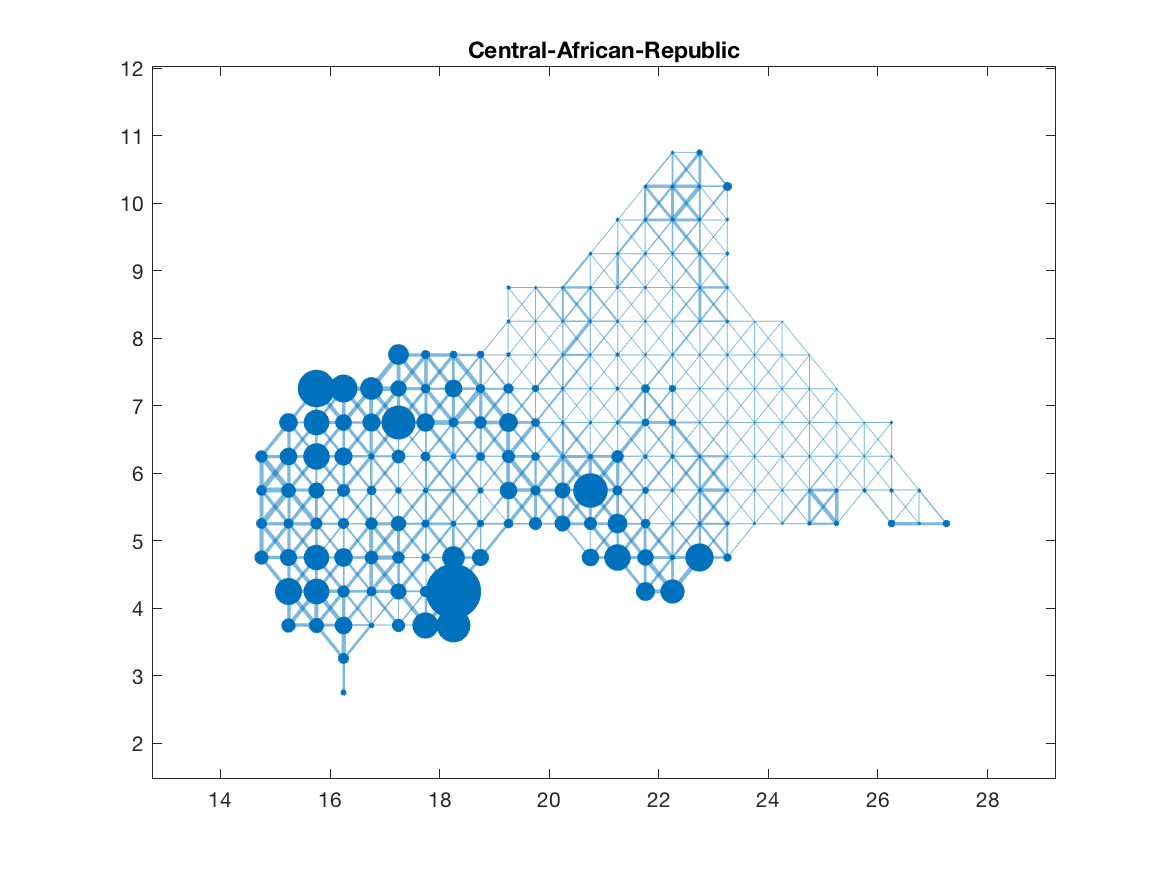
\includegraphics[width=\textwidth, trim={2cm 1cm 1.5cm 0cm},clip]{/Users/Tilmanski/Documents/UNI/MPhil/Second Year/Thesis_Git/Build/output/Matlab_graphs/Nicer_graphs/Central-African-Republic_stat.png}
\caption{pre reallocation}
\label{fig:cae_pre}
\end{subfigure}
\begin{subfigure}[c]{0.48\textwidth}
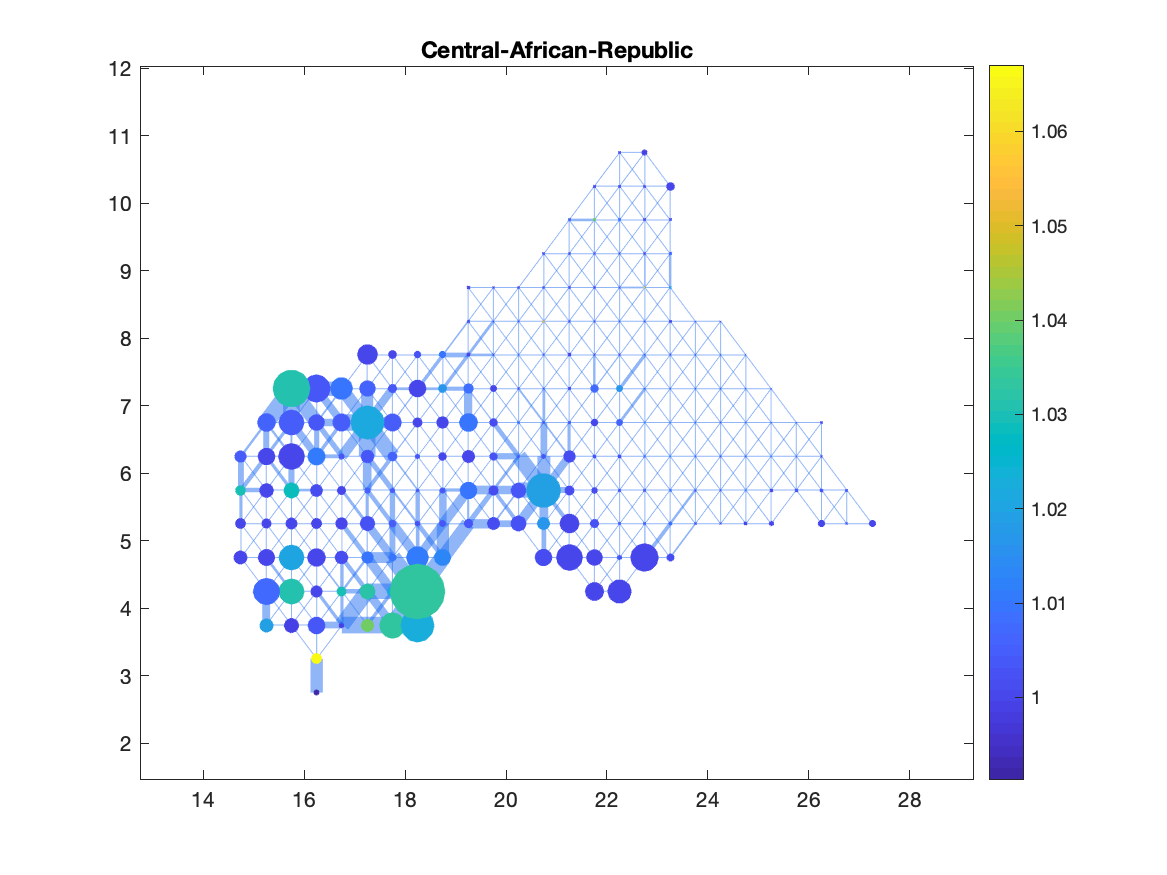
\includegraphics[width=\textwidth, trim={2cm 1cm 1.5cm 0cm},clip]{/Users/Tilmanski/Documents/UNI/MPhil/Second Year/Thesis_Git/Build/output/Matlab_graphs/Nicer_graphs/Central-African-Republic_opt.png}
\caption{post reallocation}
\label{fig:cae_post}
\end{subfigure}
\end{figure}
\end{frame}

\begin{frame}
  \frametitle{Network Reallocation}
\begin{figure}
\begin{subfigure}[c]{0.48\textwidth}
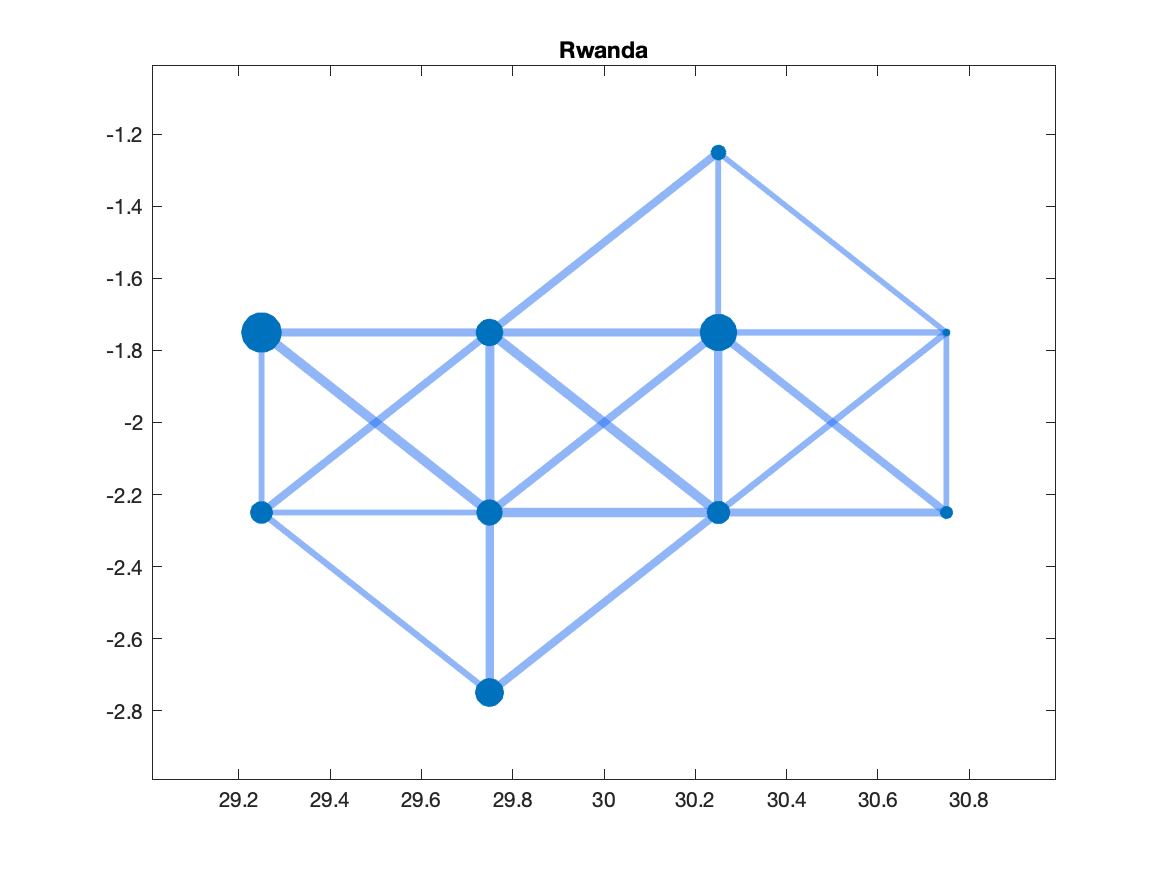
\includegraphics[width=\textwidth, trim={2cm 1cm 1.5cm 0cm},clip]{/Users/Tilmanski/Documents/UNI/MPhil/Second Year/Thesis_Git/Build/output/Matlab_graphs/Nicer_graphs/Rwanda_stat.png}
\caption{pre reallocation}
\label{fig:cae_pre}
\end{subfigure}
\begin{subfigure}[c]{0.48\textwidth}
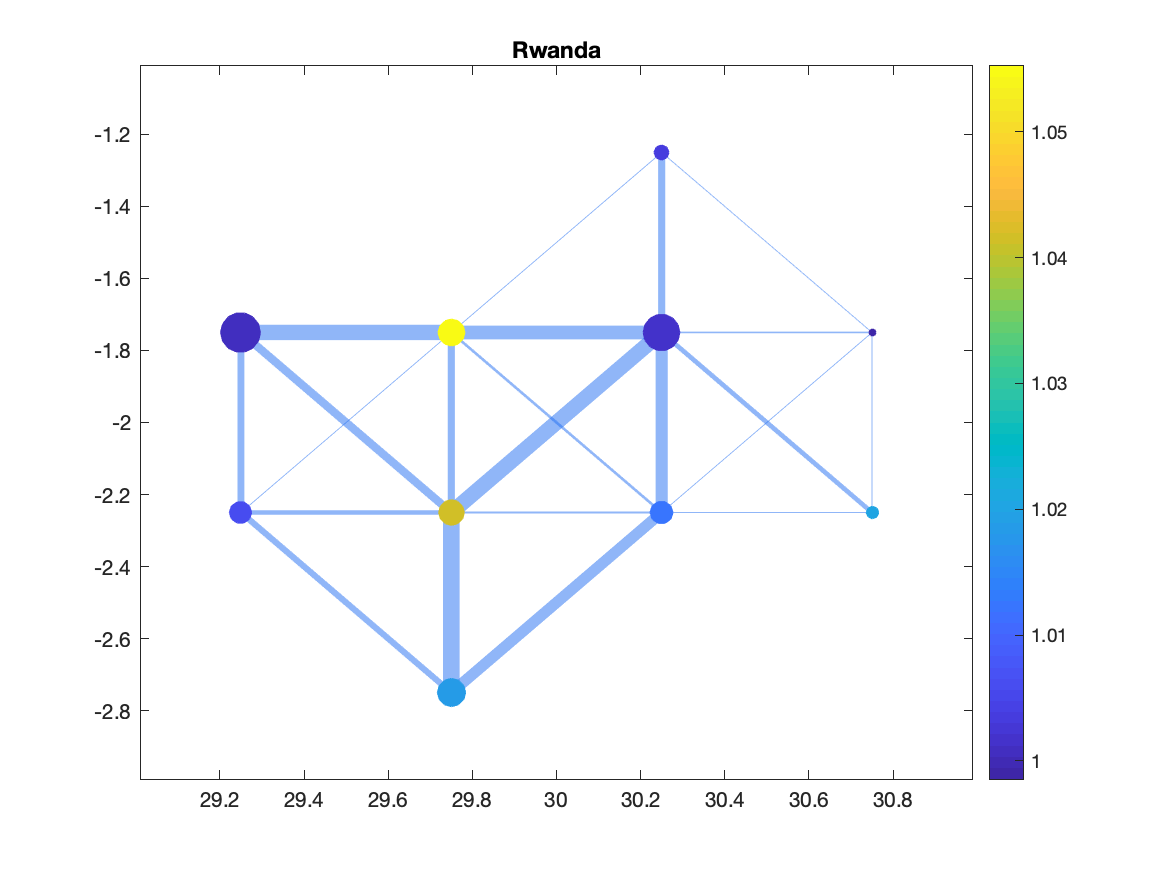
\includegraphics[width=\textwidth, trim={2cm 1cm 1.5cm 0cm},clip]{/Users/Tilmanski/Documents/UNI/MPhil/Second Year/Thesis_Git/Build/output/Matlab_graphs/Nicer_graphs/Rwanda_opt.png}
\caption{post reallocation}
\label{fig:cae_post}
\end{subfigure}
\end{figure}
\end{frame}

\begin{frame}
  \frametitle{Network Reallocation}

\begin{figure}
\begin{subfigure}[c]{0.48\textwidth}
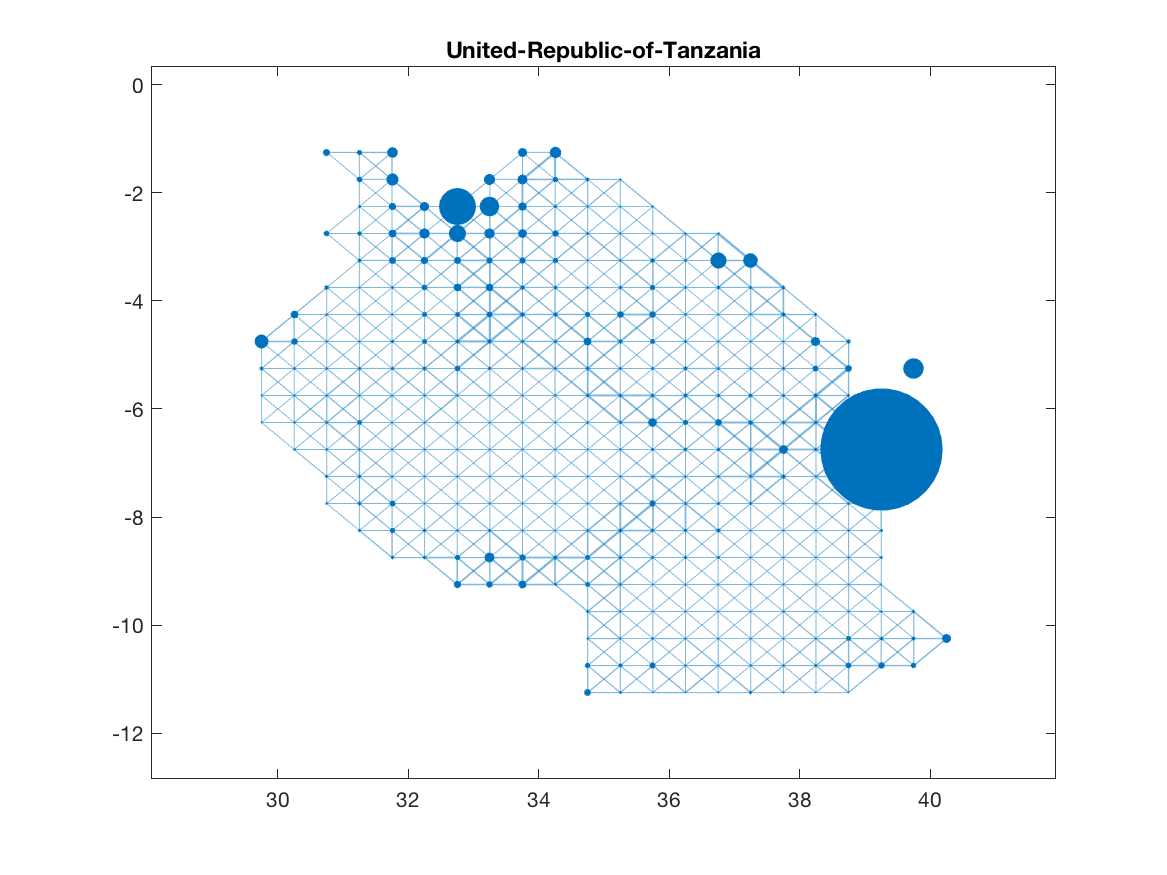
\includegraphics[width=\textwidth, trim={2cm 1cm 1.5cm 0cm},clip]{/Users/Tilmanski/Documents/UNI/MPhil/Second Year/Thesis_Git/Build/output/Matlab_graphs/Nicer_graphs/United-Republic-of-Tanzania_stat.png}
\caption{pre reallocation}
\label{fig:cae_pre}
\end{subfigure}
\begin{subfigure}[c]{0.48\textwidth}
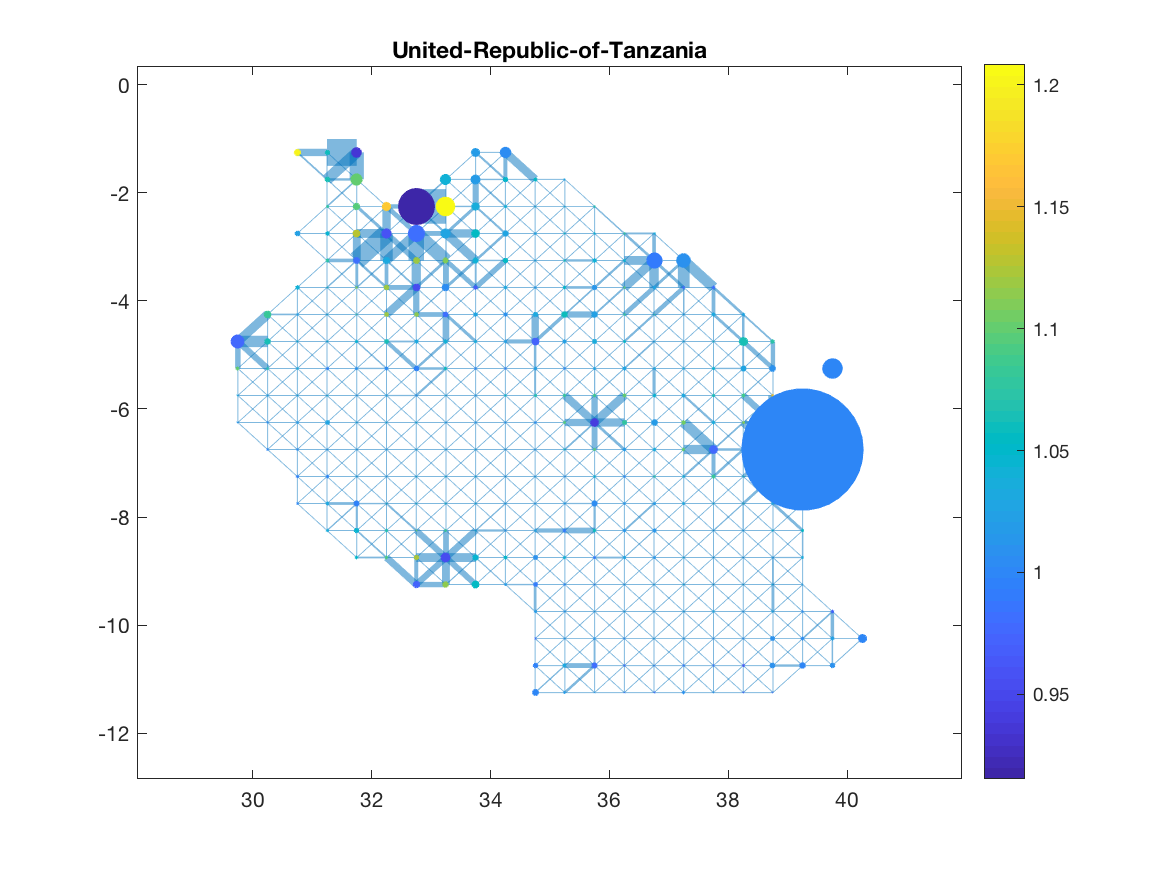
\includegraphics[width=\textwidth, trim={2cm 1cm 1.5cm 0cm},clip]{/Users/Tilmanski/Documents/UNI/MPhil/Second Year/Thesis_Git/Build/output/Matlab_graphs/Nicer_graphs/United-Republic-of-Tanzania_opt.png}
\caption{post reallocation}
\label{fig:cae_post}
\end{subfigure}
\end{figure}
\end{frame}

\begin{frame}
\label{country_map}
\frametitle{Welfare gains for entire countries}
\begin{figure}
    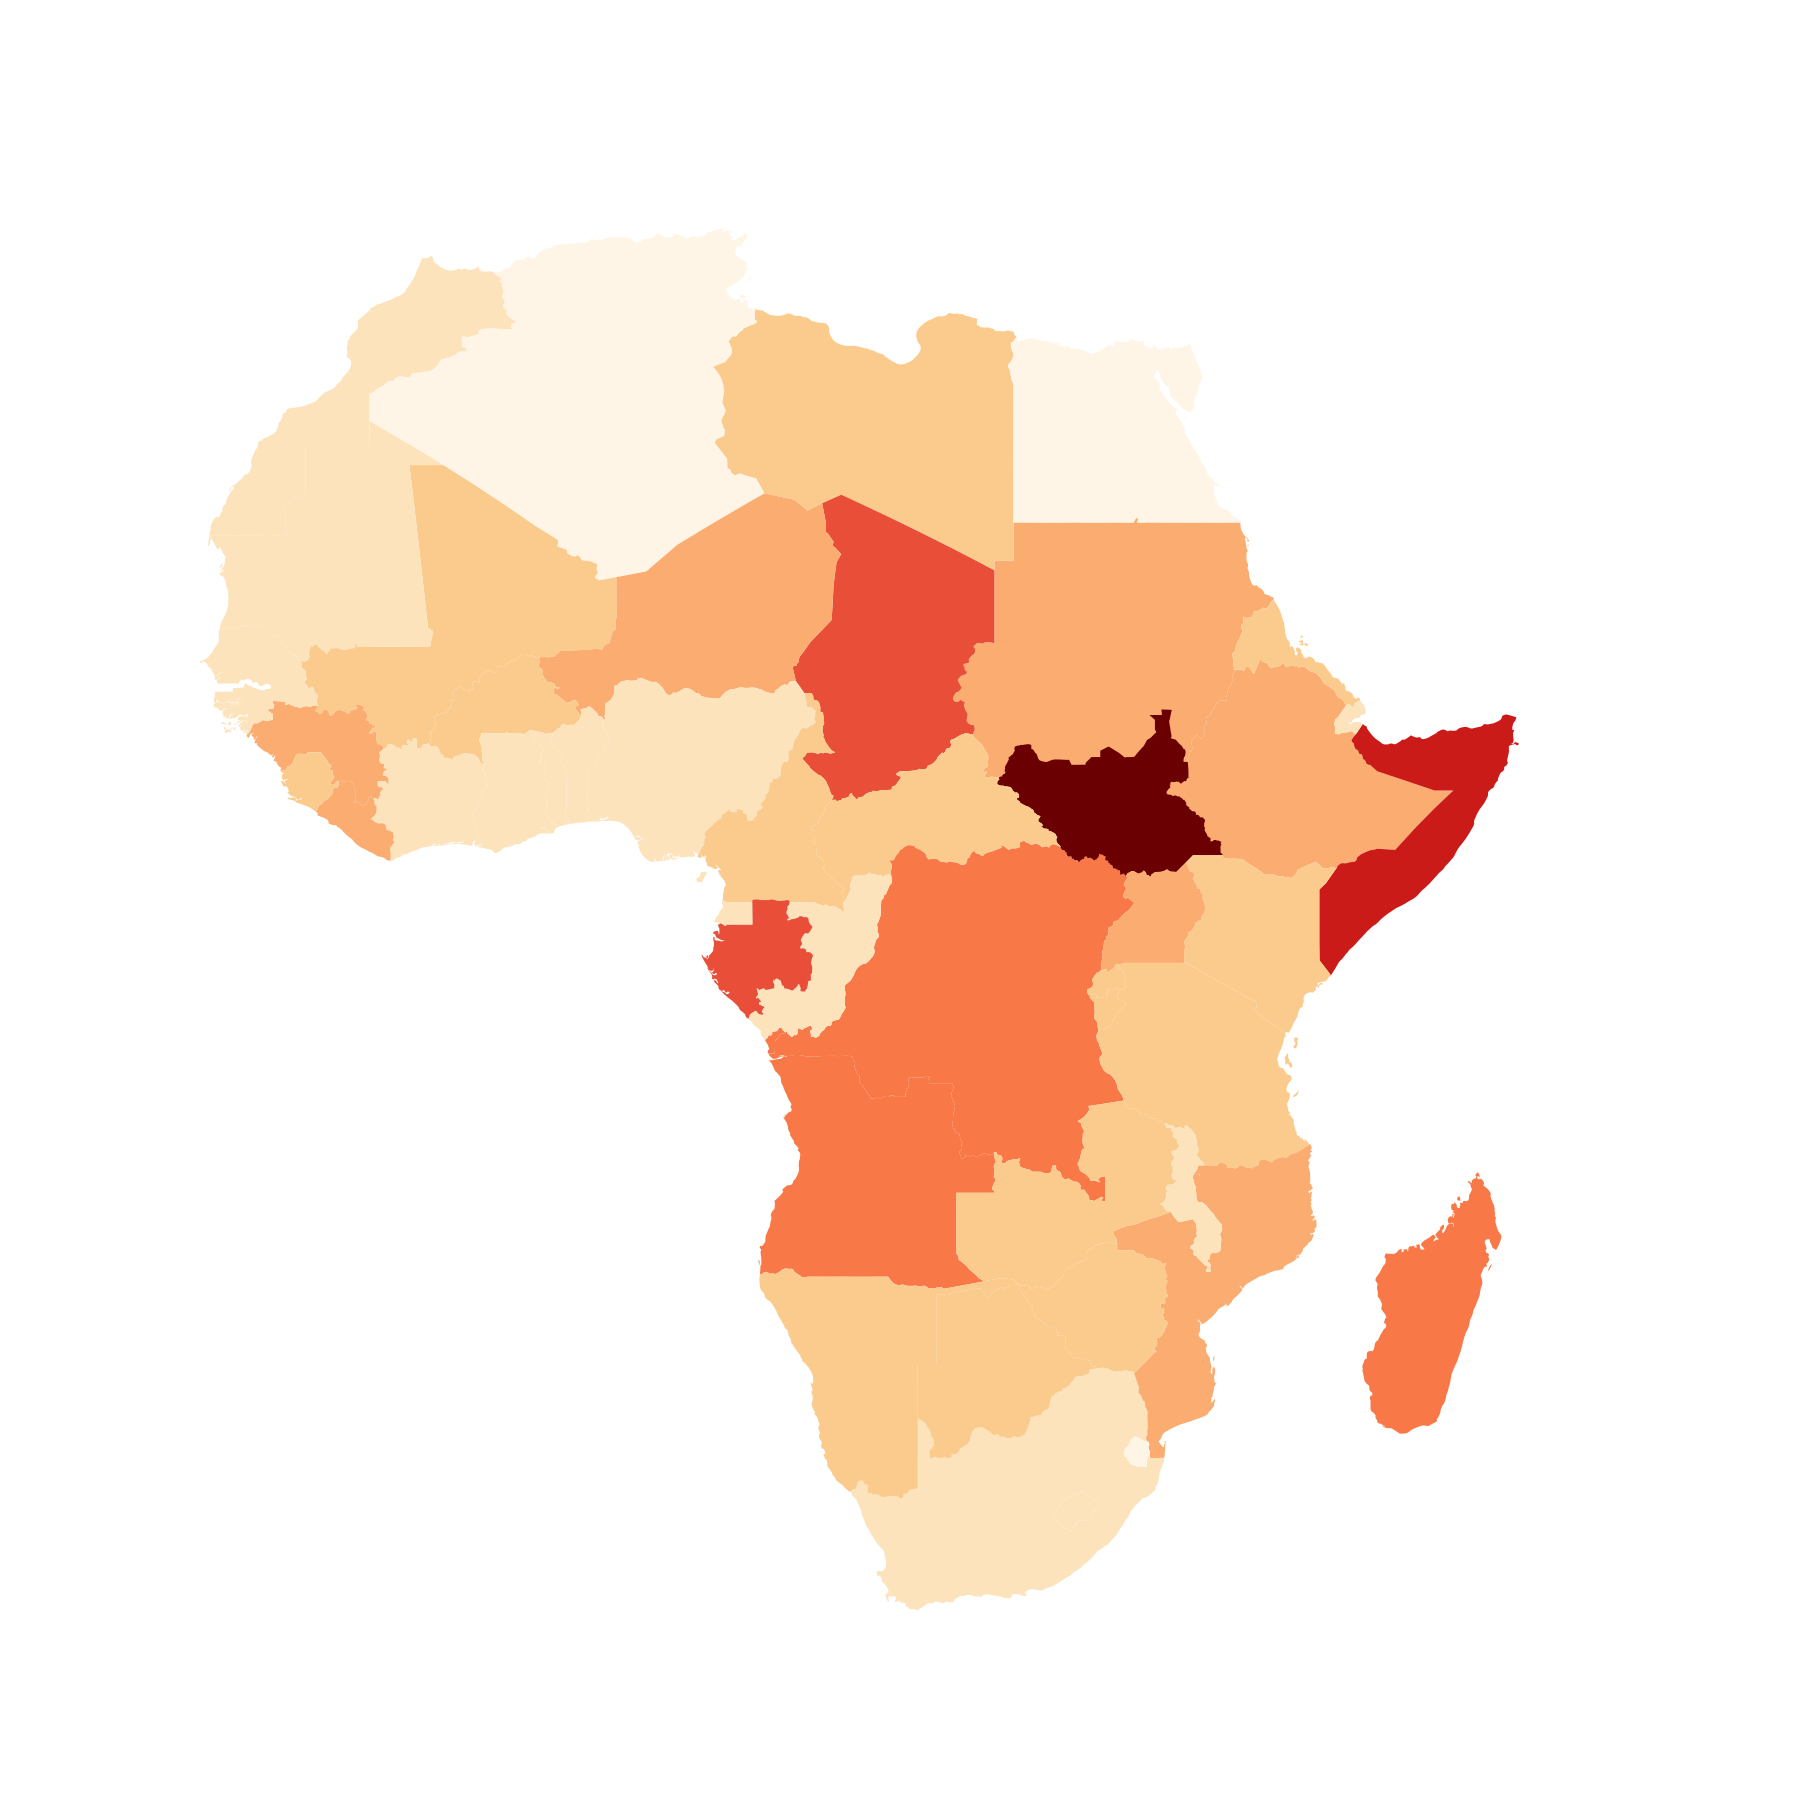
\includegraphics[width=0.65\textwidth, trim={1cm 4cm 0cm 2cm},clip]{/Users/Tilmanski/Documents/UNI/MPhil/Second Year/Thesis_Git/Analysis/output/zeta_heatmaps/African_countries_zeta.png}
    \caption{Percentage welfare gains for all countries in the sample}
  \end{figure}
\end{frame}

\begin{frame}
  \frametitle{Local Infrastructure Discrimination Index $\Lambda_{i}$}
\begin{figure}
\caption{$\Lambda_{i}$ for sample countries}
\begin{subfigure}[c]{0.32\textwidth}
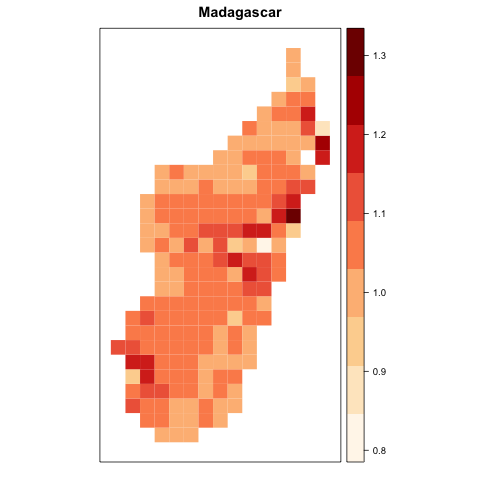
\includegraphics[width=\textwidth]{/Users/Tilmanski/Documents/UNI/MPhil/Second Year/Thesis_Git/Analysis/output/zeta_heatmaps/Madagascar_zeta.png}
\caption{Madagascar}
\label{fig:Madagascar_zeta}
\end{subfigure}
\begin{subfigure}[c]{0.32\textwidth}
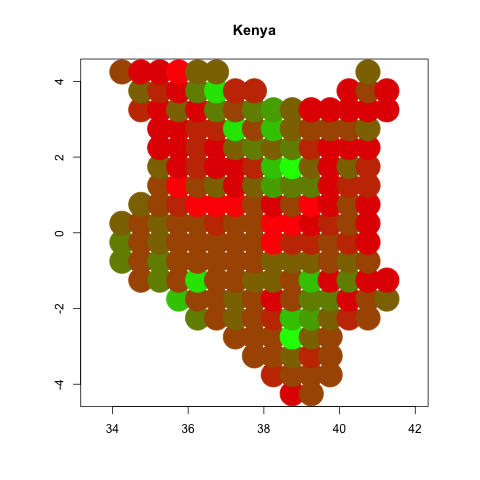
\includegraphics[width=\textwidth]{/Users/Tilmanski/Documents/UNI/MPhil/Second Year/Thesis_Git/Analysis/output/zeta_heatmaps/Kenya_zeta.png}
\caption{Kenya}
\label{fig:Kenya_zeta}
\end{subfigure}
\begin{subfigure}[c]{0.32\textwidth}
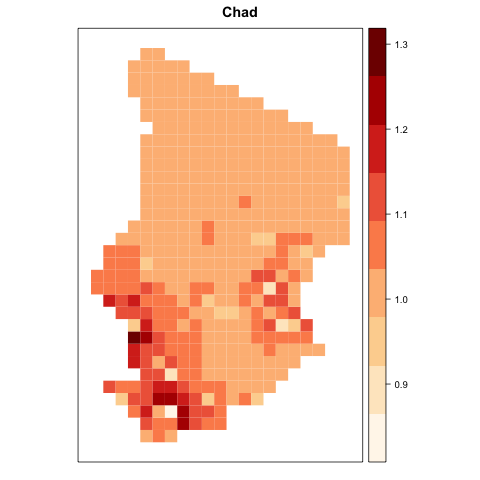
\includegraphics[width=\textwidth]{/Users/Tilmanski/Documents/UNI/MPhil/Second Year/Thesis_Git/Analysis/output/zeta_heatmaps/Chad_zeta.png}
\caption{Chad}
\label{fig:Chad_zeta}
\end{subfigure}
\end{figure}
\centering
$\Lambda_{i} = \frac{\textrm{Welfare under the optimal Infrastructure}_{i}}{\textrm{Welfare under the current Infrastructure}_{i}}$
\end{frame}

\begin{frame}
  \frametitle{$\Lambda_{i}$ for entire sample}
    \label{Grid_Cell_Map}
  \begin{figure}
    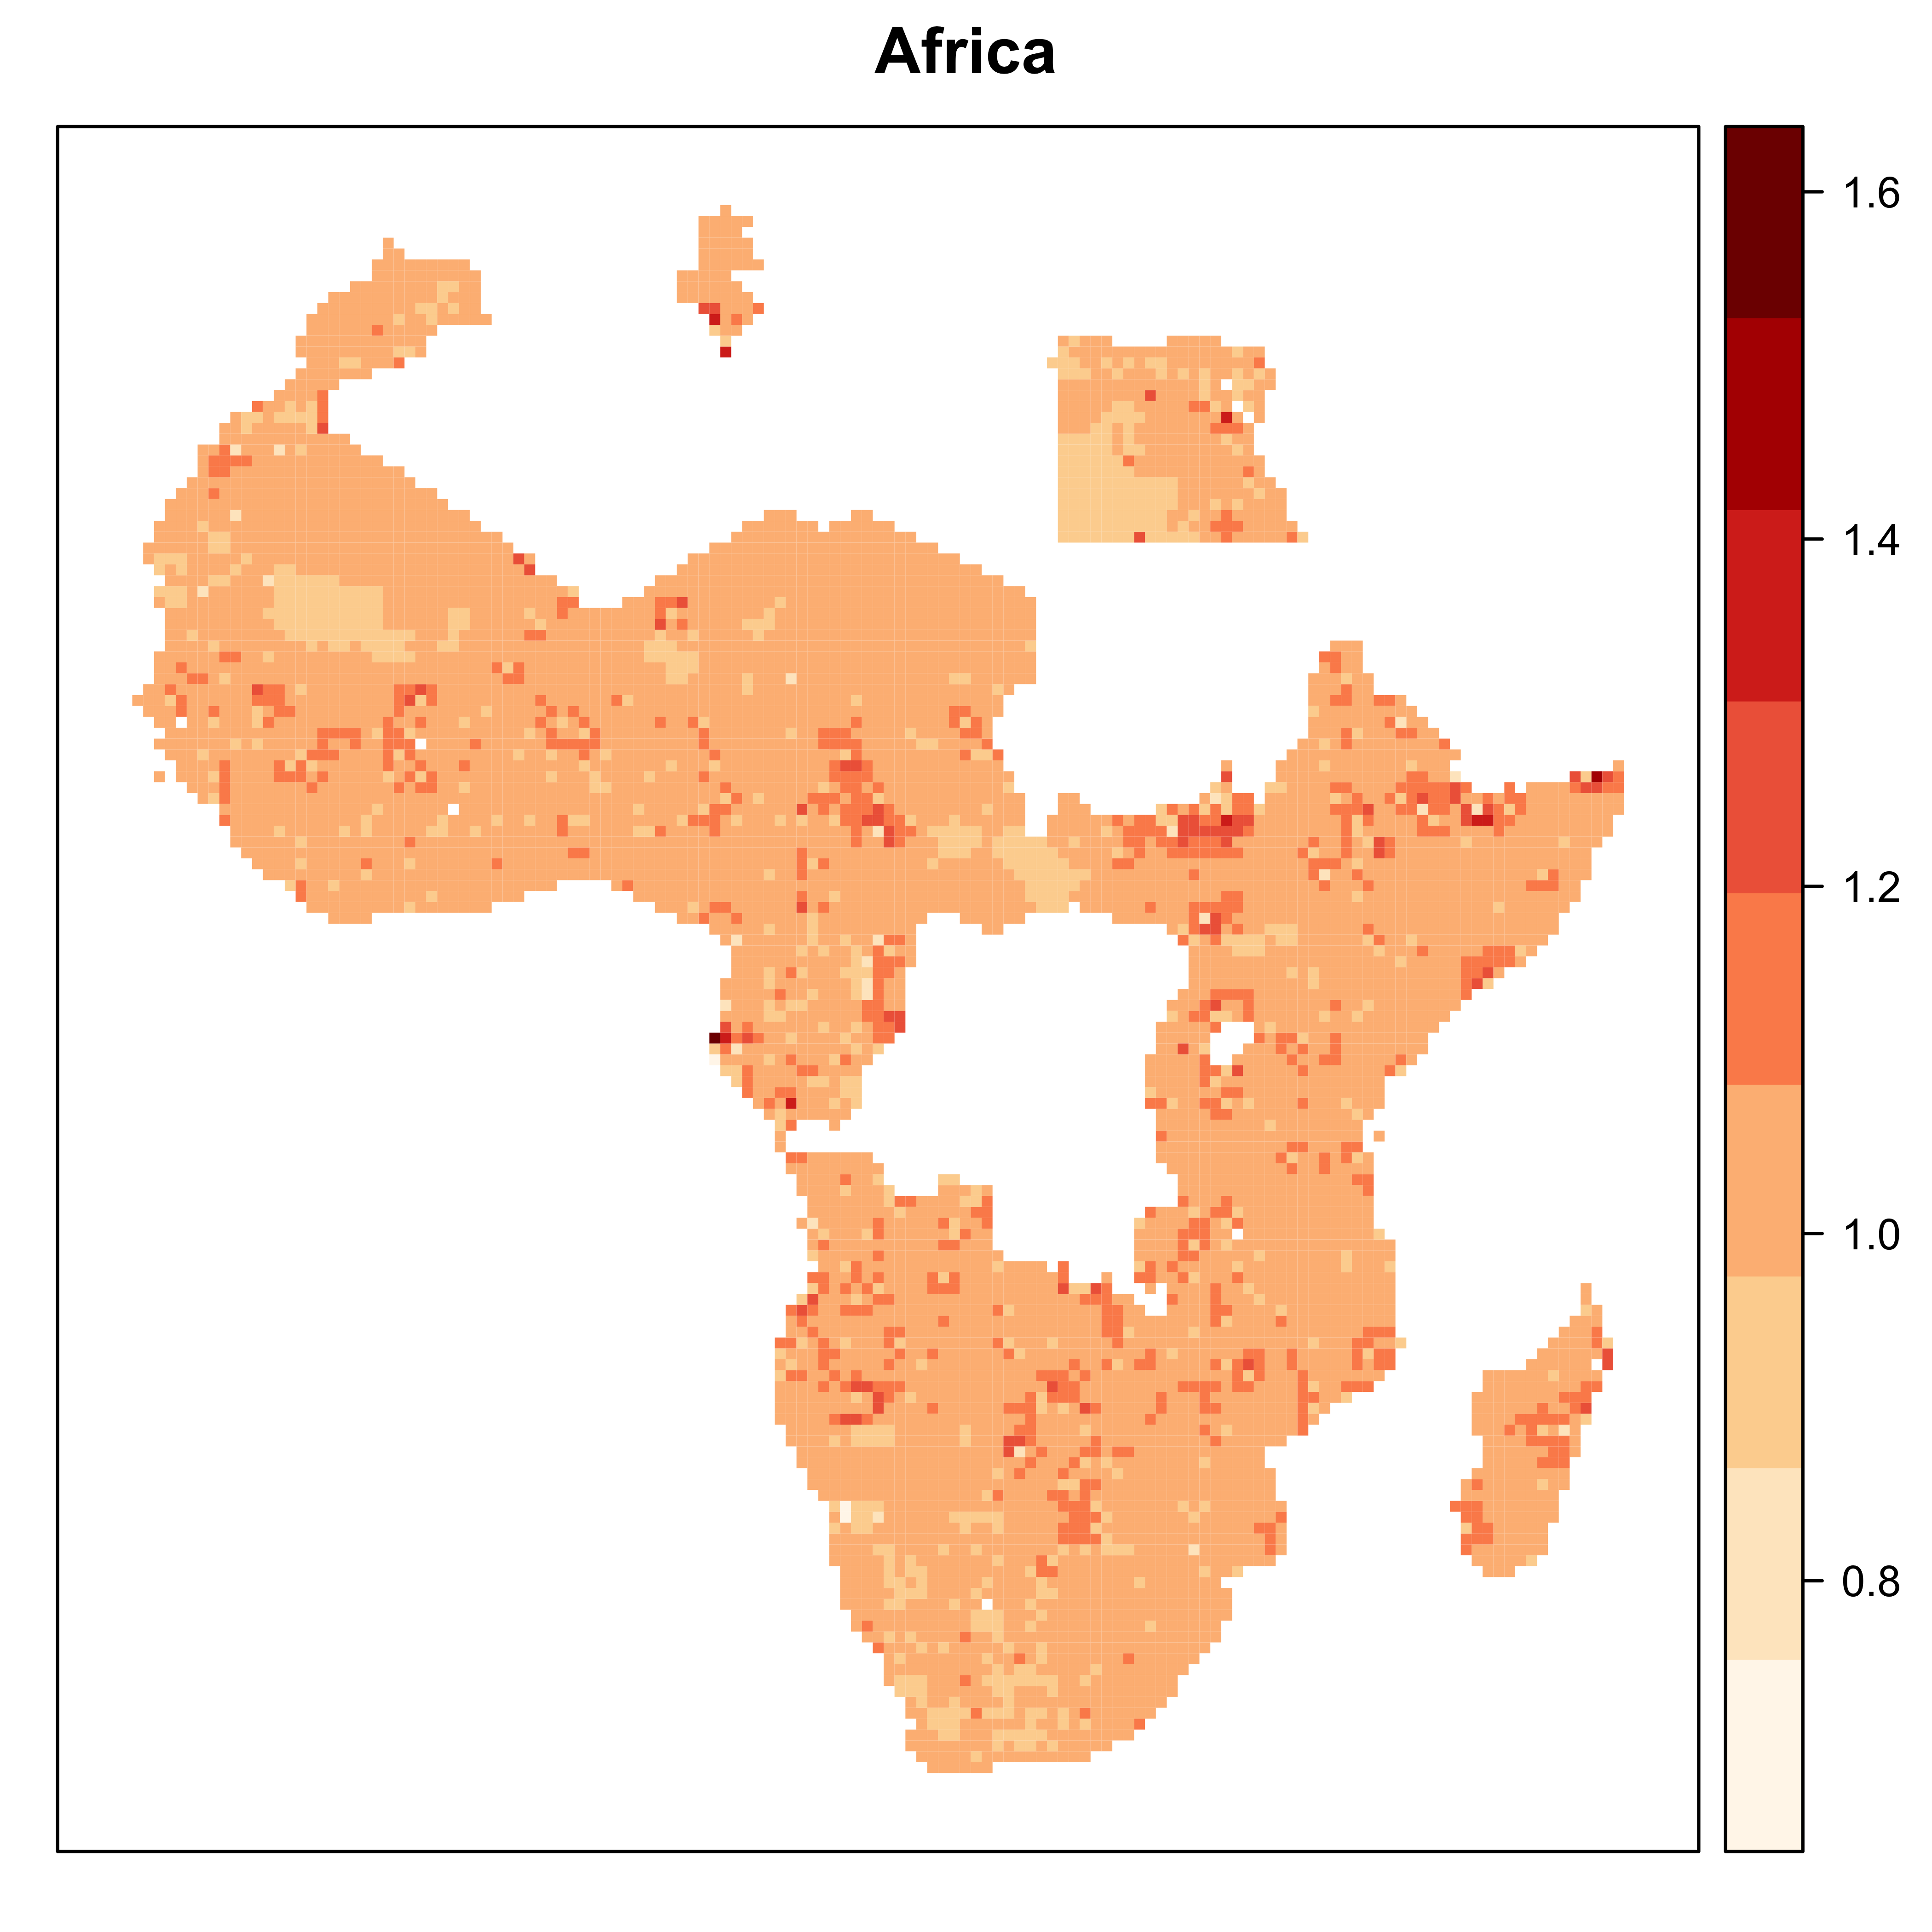
\includegraphics[width=0.65\textwidth, trim={1cm 4cm 0cm 2cm},clip]{/Users/Tilmanski/Documents/UNI/MPhil/Second Year/Thesis_Git/Analysis/output/zeta_heatmaps/African_gridcells_zeta.png}
    \caption{10,158 grid cells by $\Lambda_{i}$}
  \end{figure}
\end{frame}

\begin{frame}
  \frametitle{Steps}
  \setbeamercolor{normal text}{fg=gray,bg=}
\setbeamercolor{alerted text}{fg=black,bg=}
\usebeamercolor{normal text}
  \begin{enumerate}
    \item Network representation for all African countries
    \begin{itemize}
      \item Nodes
      \item Edges
    \end{itemize}
    \item Employ in simple trade model
    \item Reshuffle roads to get optimal network
    \item \alert{Analyse patterns of reshuffling}
  \end{enumerate}
\end{frame}

\begin{frame}
Why do some areas have too few roads while others have too many?
\end{frame}

\begin{frame}
\frametitle{Lasting impact of Colonial Railroads}
\begin{figure}
\centering
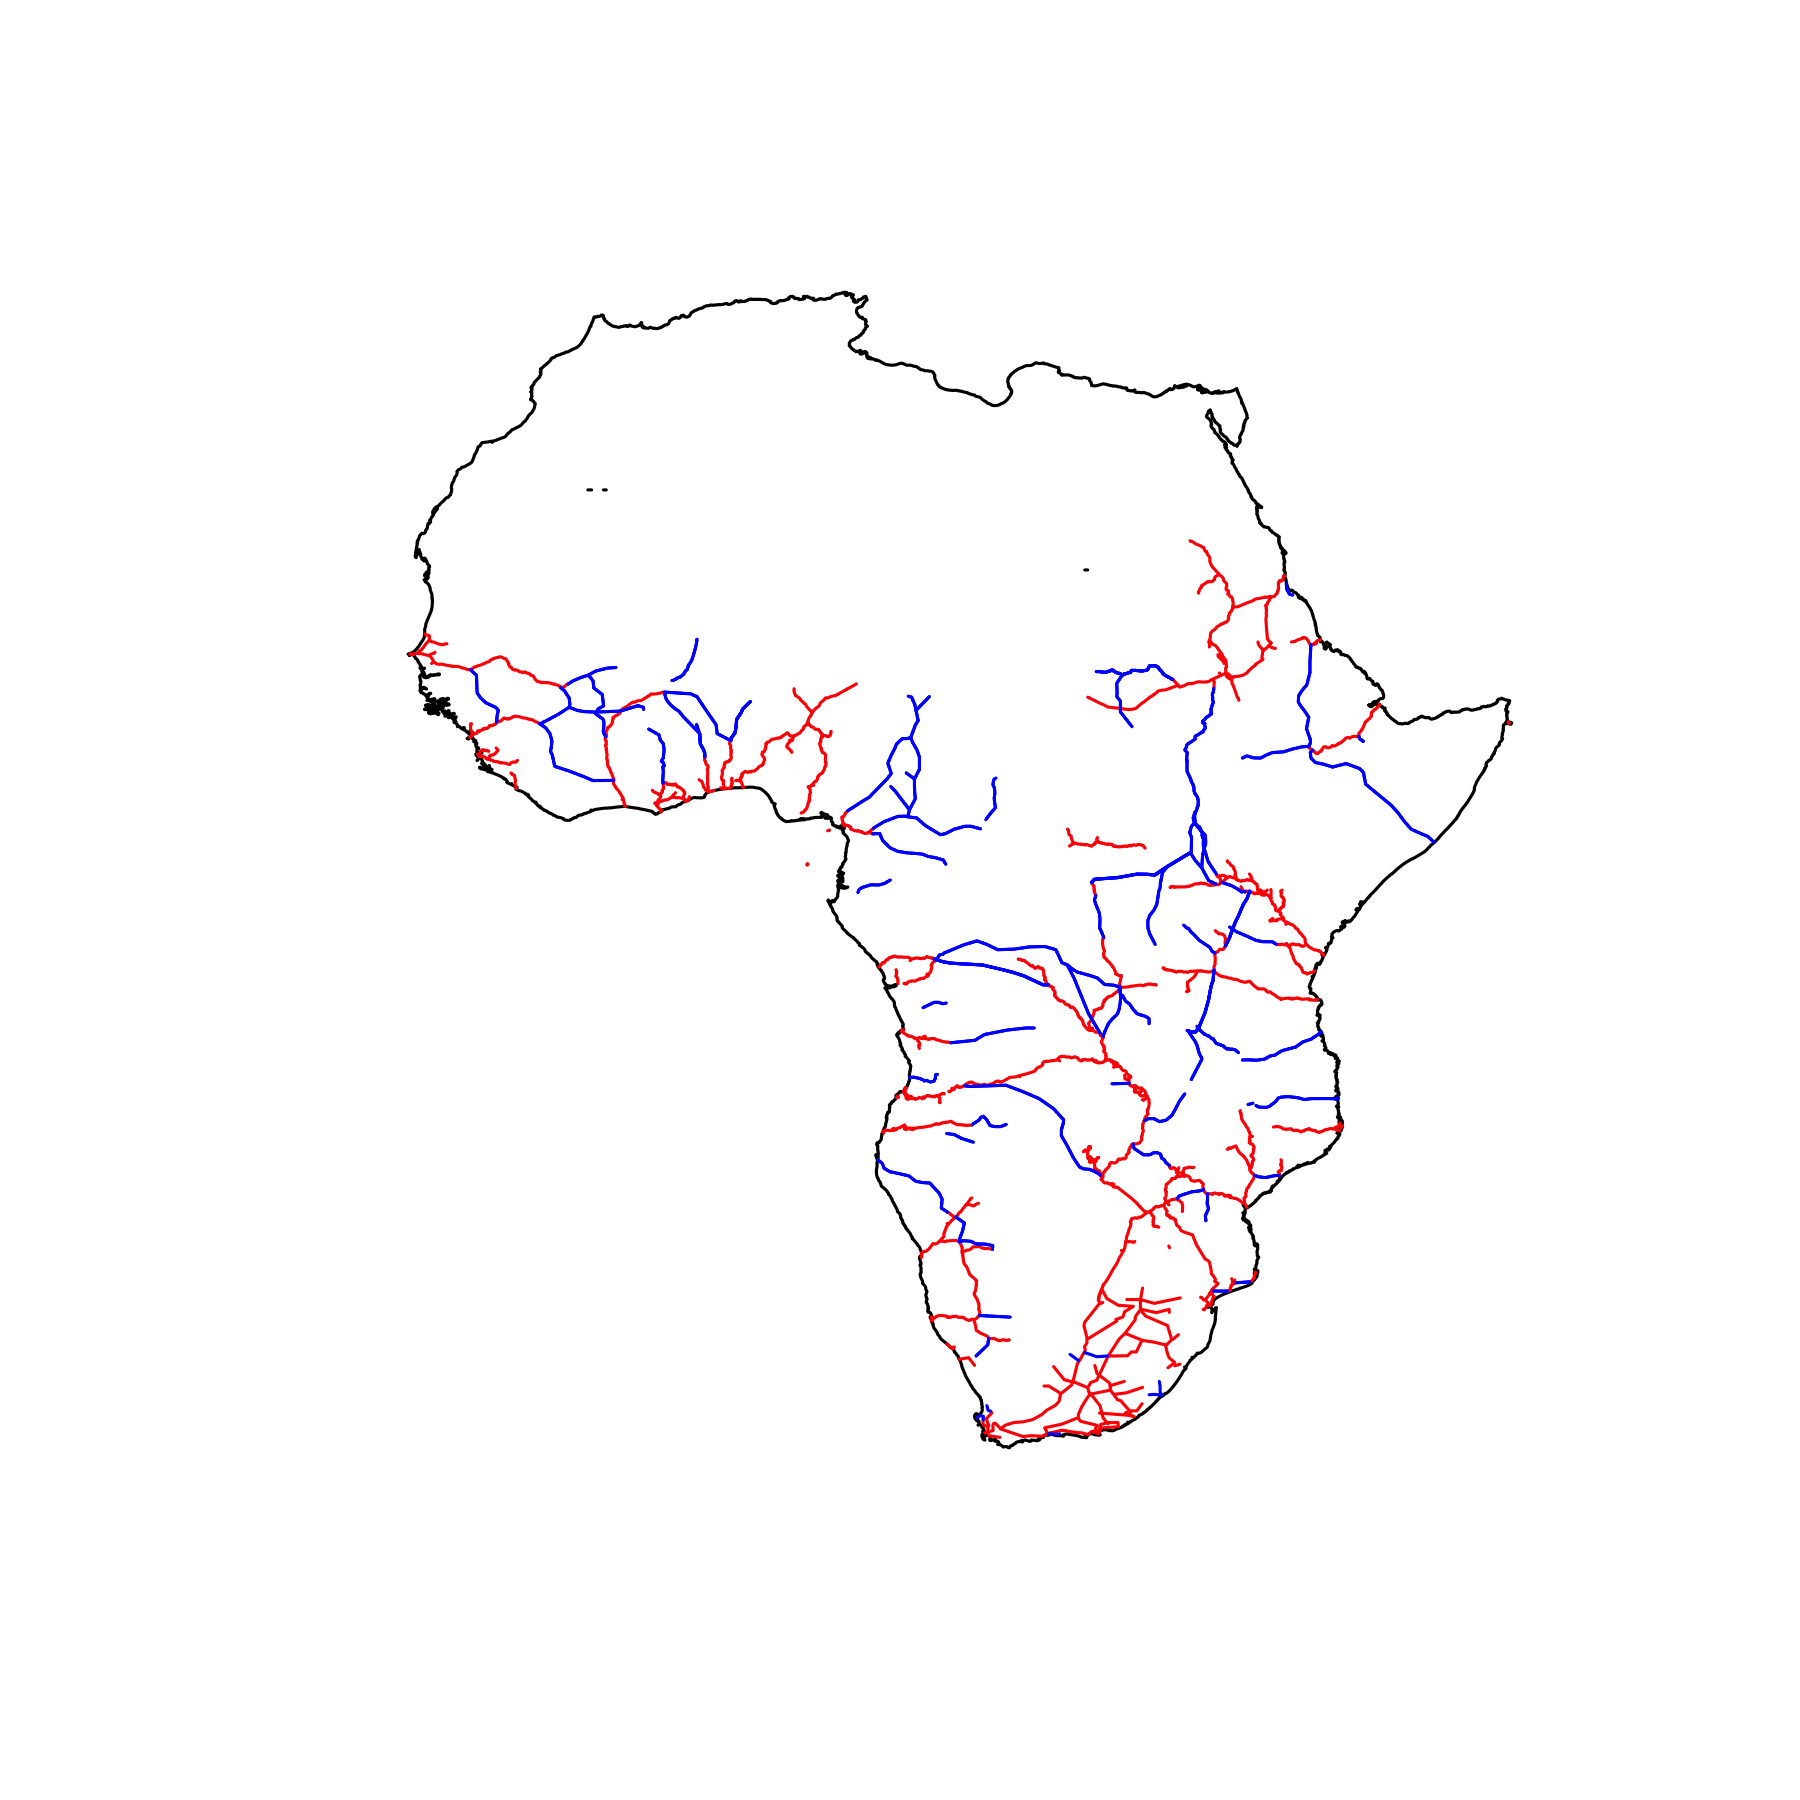
\includegraphics[width=0.6\textwidth,trim={10cm 11cm 6cm 10cm},clip]{/Users/Tilmanski/Documents/UNI/MPhil/Second Year/Thesis_Git/Analysis/output/other_maps/all_rails.png}
\caption{Colonial Rails (red) and Placebo Rails (blue)}
\label{fig:Rail Maps}
\end{figure}
  \tiny Source: Jedwab \& Moradi (2016) and own digitisations
\end{frame}

\begin{frame}
\frametitle{Lasting impact of Colonial Railroads}
\begin{table}[t] \centering
  \caption{Colonial Railroads and Local Infrastructure Discrimination Index}
  \label{tab:RailKM_zeta}
  \resizebox{\textwidth}{!}{

  \begin{tabular}{@{\extracolsep{5pt}}lcccccccc}
  \\[-1.8ex]\hline
  \hline \\[-1.8ex]
   & \multicolumn{8}{c}{\textit{Dependent variable:}} \\
  \cline{2-9}
  \\[-1.8ex] & \multicolumn{8}{c}{Local Infrastructure Discrimination Index $\Lambda_{i}$} \\
  \\[-1.8ex] & (1) & (2) & (3) & (4) & (5) & (6) & (7) & (8)\\
  \hline \\[-1.8ex]
   KM of Colonial Railroads & $-$0.0002$^{***}$ & $-$0.0001$^{***}$ & $-$0.0002$^{***}$ & $-$0.0002$^{***}$ &  &  &  &  \\
  & (0.0001) & (0.0001) & (0.0001) & (0.0001) &  &  &  &  \\
    & & & & & & & & \\
   KM of Colonial Placebo Railroads &  &  &  &  & 0.00004 & $-$0.0002 & $-$0.0002 & $-$0.0003 \\
  &  &  &  &  & (0.0003) & (0.0003) & (0.0003) & (0.0003) \\
    & & & & & & & & \\
  \hline \\[-1.8ex]
  Country FE &  & Yes & Yes & Yes &  & Yes & Yes & Yes \\
  Geographic controls &  &  & Yes & Yes &  &  & Yes & Yes \\
  Simulation controls &  &  &  & Yes &  &  &  & Yes \\
  Observations & 10,158 & 10,158 & 10,158 & 10,158 & 10,158 & 10,158 & 10,158 & 10,158 \\
  R$^{2}$ & 0.001 & 0.099 & 0.124 & 0.126 & 0.00000 & 0.098 & 0.122 & 0.124 \\
  \hline
  \hline \\[-1.8ex]
  \textit{Note:}  & \multicolumn{8}{r}{$^{*}$p$<$0.1; $^{**}$p$<$0.05; $^{***}$p$<$0.01} \\
  \end{tabular}

}

\end{table}
\end{frame}


\begin{frame}
\frametitle{Regional Favoritism}
\begin{figure}
\centering
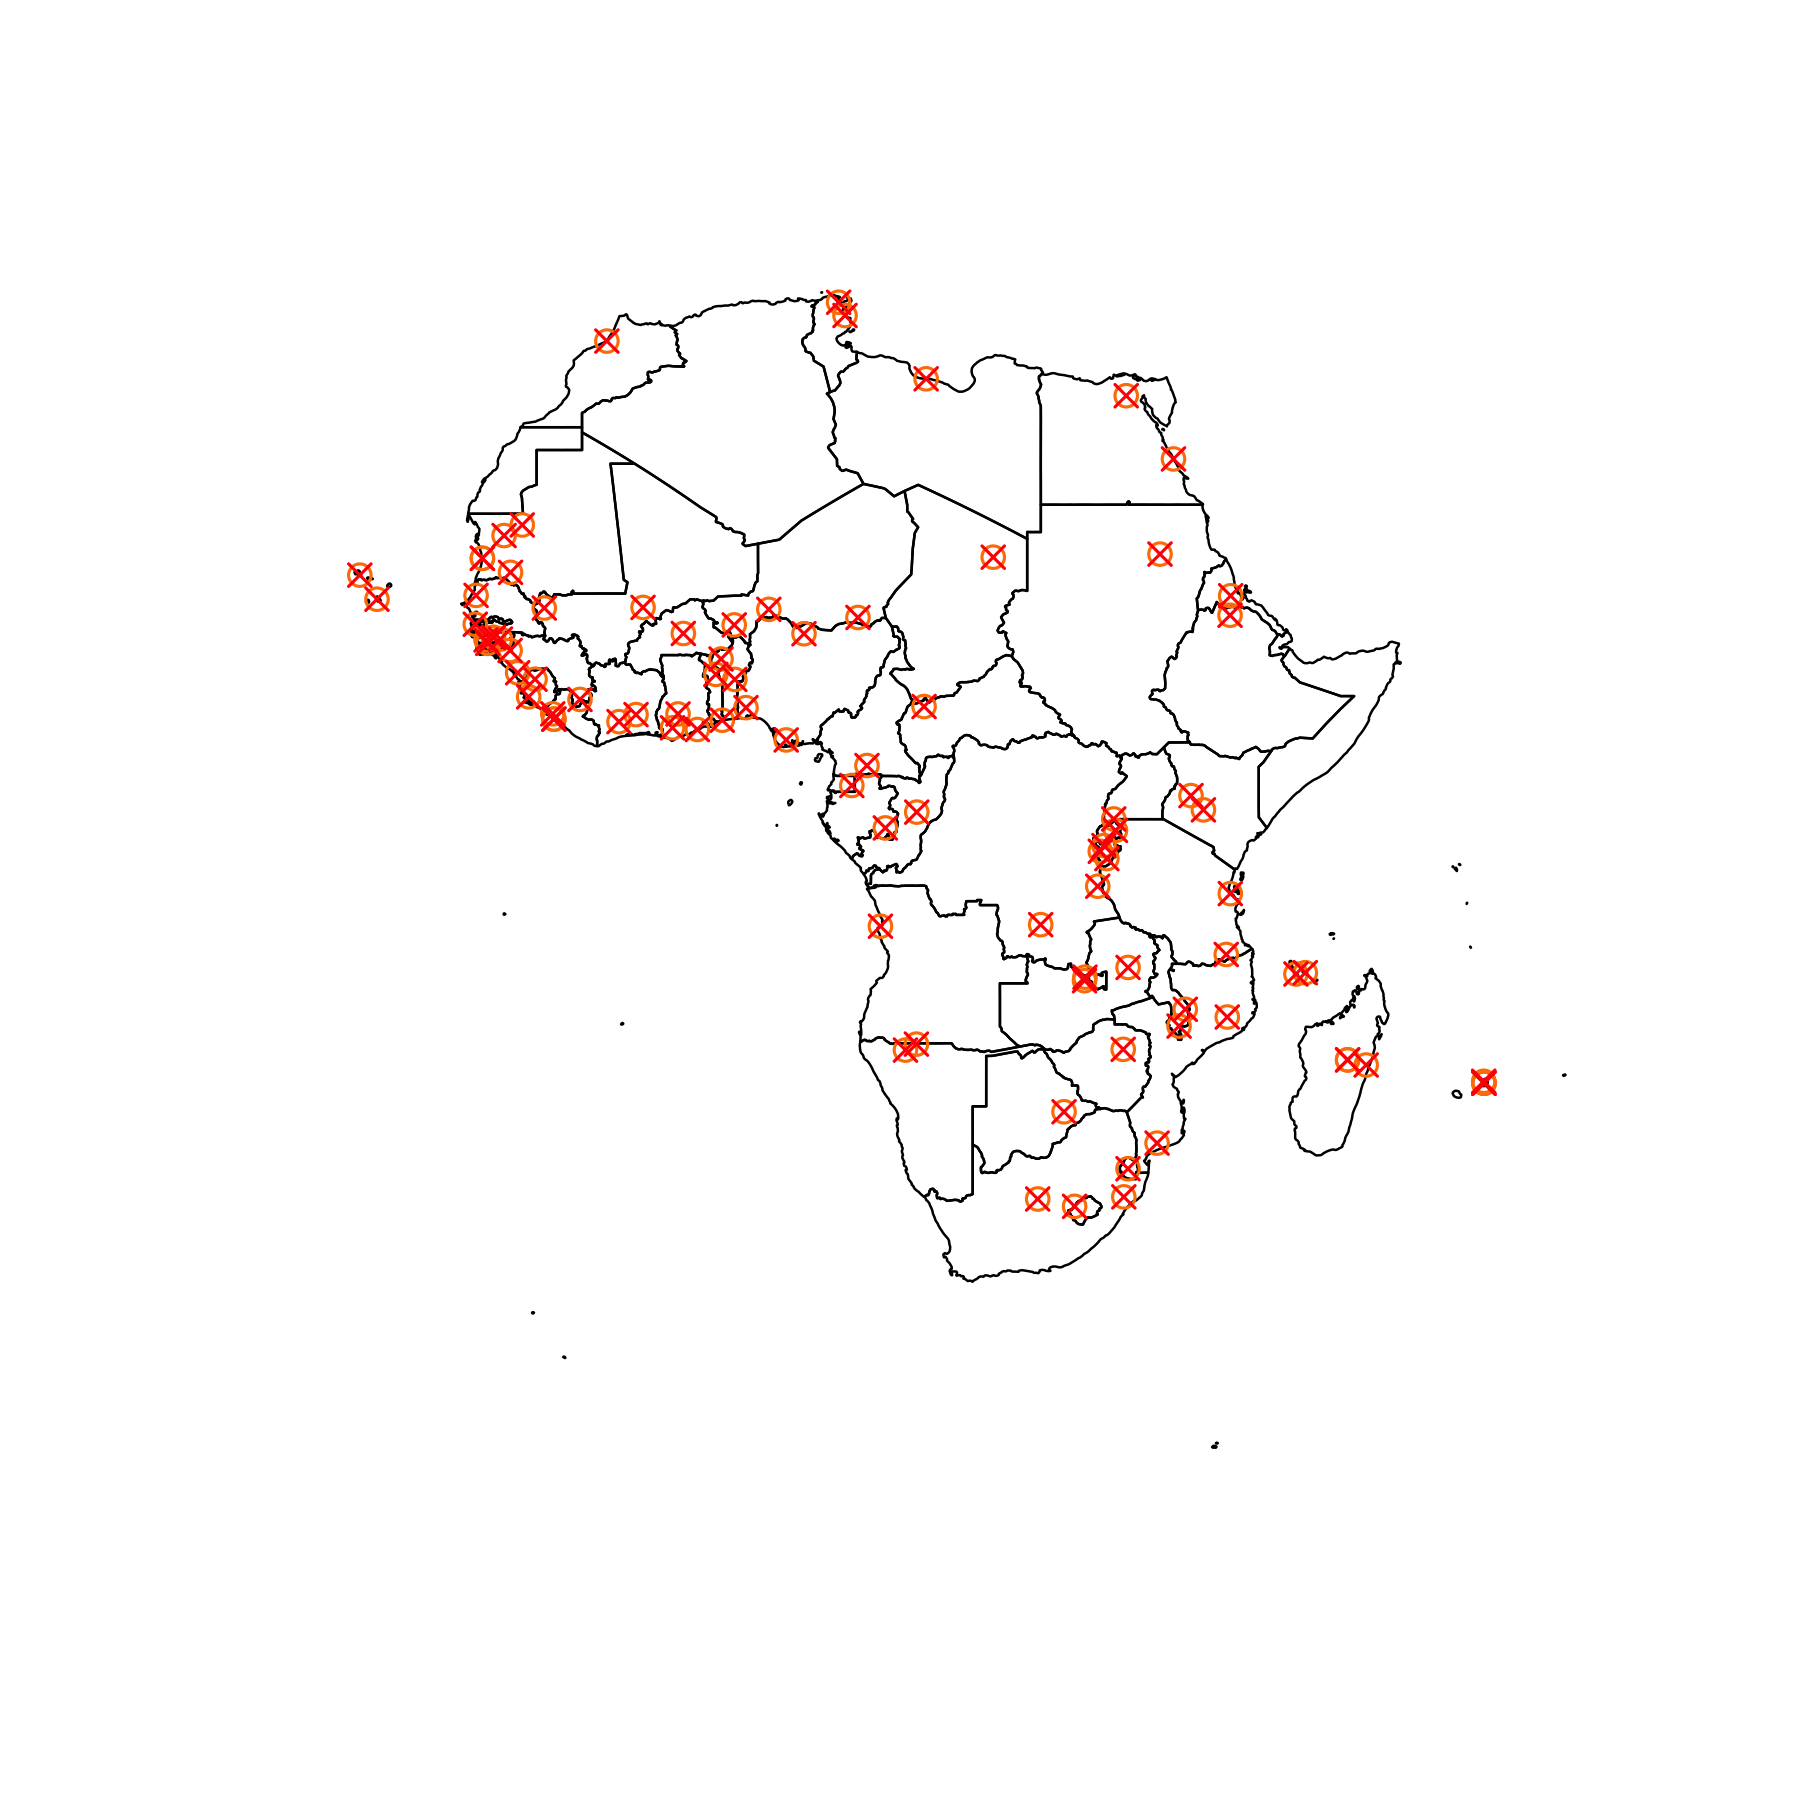
\includegraphics[width=0.6\textwidth,trim={15cm 16cm 10cm 8cm},clip]{/Users/Tilmanski/Documents/UNI/MPhil/Second Year/Thesis_Git/Analysis/output/other_maps/birthplaces.png}
\caption{Birthplaces of African heads of state since 1970}
\label{fig:birthplaces}
\end{figure}
\end{frame}

\begin{frame}
\frametitle{Regional Favoritism}
\begin{table}[!t] \centering
  \label{tab:favoritism}
  \resizebox{\textwidth}{!}{


  \begin{tabular}{@{\extracolsep{5pt}}lcccccccc}
  \\[-1.8ex]\hline
  \hline \\[-1.8ex]
   & \multicolumn{8}{c}{\textit{Dependent variable: Local Infrastructure Discrimination Index $\Lambda$}} \\
  \cline{2-9} \\[-1.8ex]
& \multicolumn{5}{c}{Full Sample} & \multicolumn{3}{c}{Excluding Capitals} \\
  \cline{2-6}   \cline{7-9}
  \\[-1.8ex] & (1) & (2) & (3) & (4) & (5) & (6) & (7) & (8)\\
  \hline \\[-1.8ex]
  Years in Power & $-$0.001$^{***}$ & $-$0.001$^{***}$ & $-$0.001$^{***}$ &  &  & $-$0.001$^{***}$ & $-$0.001$^{**}$ &  \\
   & (0.0003) & (0.0002) & (0.0004) &  &  & (0.0003) & (0.0004) &  \\
   & & & & & & & & \\
  Years in Power $\times$ Democracy &  &  & $-$0.0001 &  &  &  & $-$0.0002 &  \\
   &  &  & (0.001) &  &  &  & (0.001) &  \\
   & & & & & & & & \\
  In Power Dummy &  &  &  & $-$0.024$^{***}$ & $-$0.025$^{***}$ &  &  & $-$0.026$^{***}$ \\
   &  &  &  & (0.006) & (0.006) &  &  & (0.007) \\
   & & & & & & & & \\
 \hline
 Country FE & Yes & Yes & Yes & Yes & Yes & Yes & Yes & Yes \\
 Geographic controls & Yes & Yes & Yes & Yes & Yes & Yes & Yes & Yes \\
 Simulation controls &  & Yes & Yes &  & Yes & Yes & Yes & Yes \\
 Observations & 10,066 & 10,066 & 10,066 & 10,066 & 10,066 & 10,019 & 10,019 & 10,019 \\
 R$^{2}$ & 0.124 & 0.125 & 0.125 & 0.124 & 0.126 & 0.128 & 0.128 & 0.128 \\
 \hline
 \hline \\[-1.8ex]
 \textit{Note:}  & \multicolumn{8}{r}{$^{*}$p$<$0.1; $^{**}$p$<$0.05; $^{***}$p$<$0.01} \\
 \end{tabular}

}

\end{table}

\end{frame}


\begin{frame}
\frametitle{Ethnic Relations}
\begin{figure}
\centering
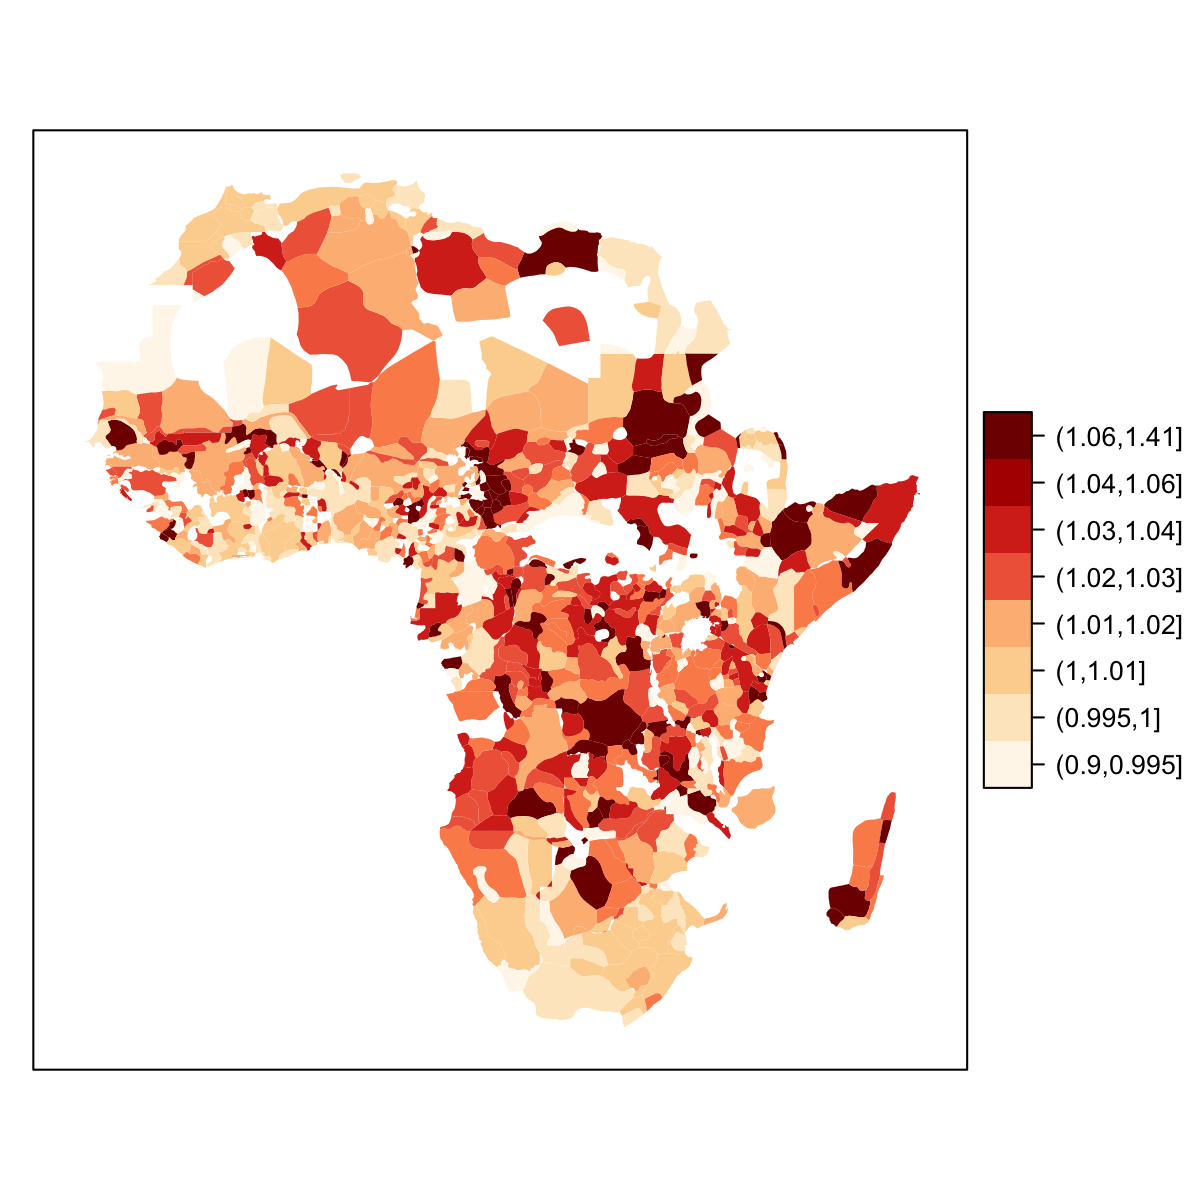
\includegraphics[width=0.65\textwidth,trim={1cm 4cm 0cm 4.5cm},clip]{/Users/Tilmanski/Documents/UNI/MPhil/Second Year/Thesis_Git/Analysis/output/other_maps/ethnicity_zeta.png}
\caption{$\Lambda_{h}$ over ethnic homelands}
\label{fig:ethnicities}
\end{figure}
\end{frame}

\begin{frame}
\frametitle{Ethnic Relations}
\begin{table}[t] \centering
  \caption{Null Effect of Ethnic Discrimination}
  \label{tab:Ethn_discrimination}
  \resizebox{\textwidth}{!}{


  \begin{tabular}{@{\extracolsep{5pt}}lcccccccc}
  \\[-1.8ex]\hline
  \hline \\[-1.8ex]
   & \multicolumn{8}{c}{\textit{Dependent variable: Local Infrastructure Discrimination Index $\Lambda_{h}$}} \\
  \cline{2-9}
  \\[-1.8ex] & (1) & (2) & (3) & (4) & (5) & (6) & (7) & (8)\\
  \hline \\[-1.8ex]
   Ethnicity discriminated against 1960--2010 & $-$0.001 & $-$0.001 &  &  &  &  &  &  \\
  & (0.008) & (0.007) &  &  &  &  &  &  \\
    & & & & & & & & \\
   Ethnicity excluded from the &  &  & $-$0.006 & $-$0.005 &  &  &  &  \\
    \hspace*{3mm} central government 1960--2010 &  &  & (0.005) & (0.005) &  &  &  &  \\
    & & & & & & & & \\
   Ethnicity involved in an &  &  &  &  & 0.002 & 0.002 &  &  \\
    \hspace*{3mm}  ethnic war 1960--2010 &  &  &  &  & (0.008) & (0.008) &  &  \\
    & & & & & & & & \\
   Ethnicity split by colonial borders &  &  &  &  &  &  & $-$0.002 & $-$0.002 \\
   &  &  &  &  &  &  & (0.004) & (0.004) \\
    & & & & & & & & \\
  \hline \\[-1.8ex]
  Country FE & Yes & Yes & Yes & Yes & Yes & Yes & Yes & Yes \\
  Geographic controls & Yes & Yes & Yes & Yes & Yes & Yes & Yes & Yes \\
  Simulation controls &  & Yes &  & Yes &  & Yes &  & Yes \\
  Observations & 496 & 496 & 496 & 496 & 496 & 496 & 932 & 932 \\
  R$^{2}$ & 0.156 & 0.166 & 0.158 & 0.168 & 0.156 & 0.167 & 0.164 & 0.167 \\
  \hline
  \hline \\[-1.8ex]
  \textit{Note:}  & \multicolumn{8}{r}{$^{*}$p$<$0.1; $^{**}$p$<$0.05; $^{***}$p$<$0.01} \\
  \end{tabular}

}
\end{table}
% \centering
% \footnotesize
%
% Estimating Equation $\Lambda_{h,c} = \beta EthnicDiscrimination_{h,c} + \textbf{X}_{h,c}\gamma + \delta_{c} + \epsilon_{h,c}$
\end{frame}

\begin{frame}
\frametitle{Does Aid go into the right locations?}
\begin{figure}[t]
\centering
\caption{Spatial Distribution of Development Aid Projects}

\begin{subfigure}[c]{0.48\textwidth}
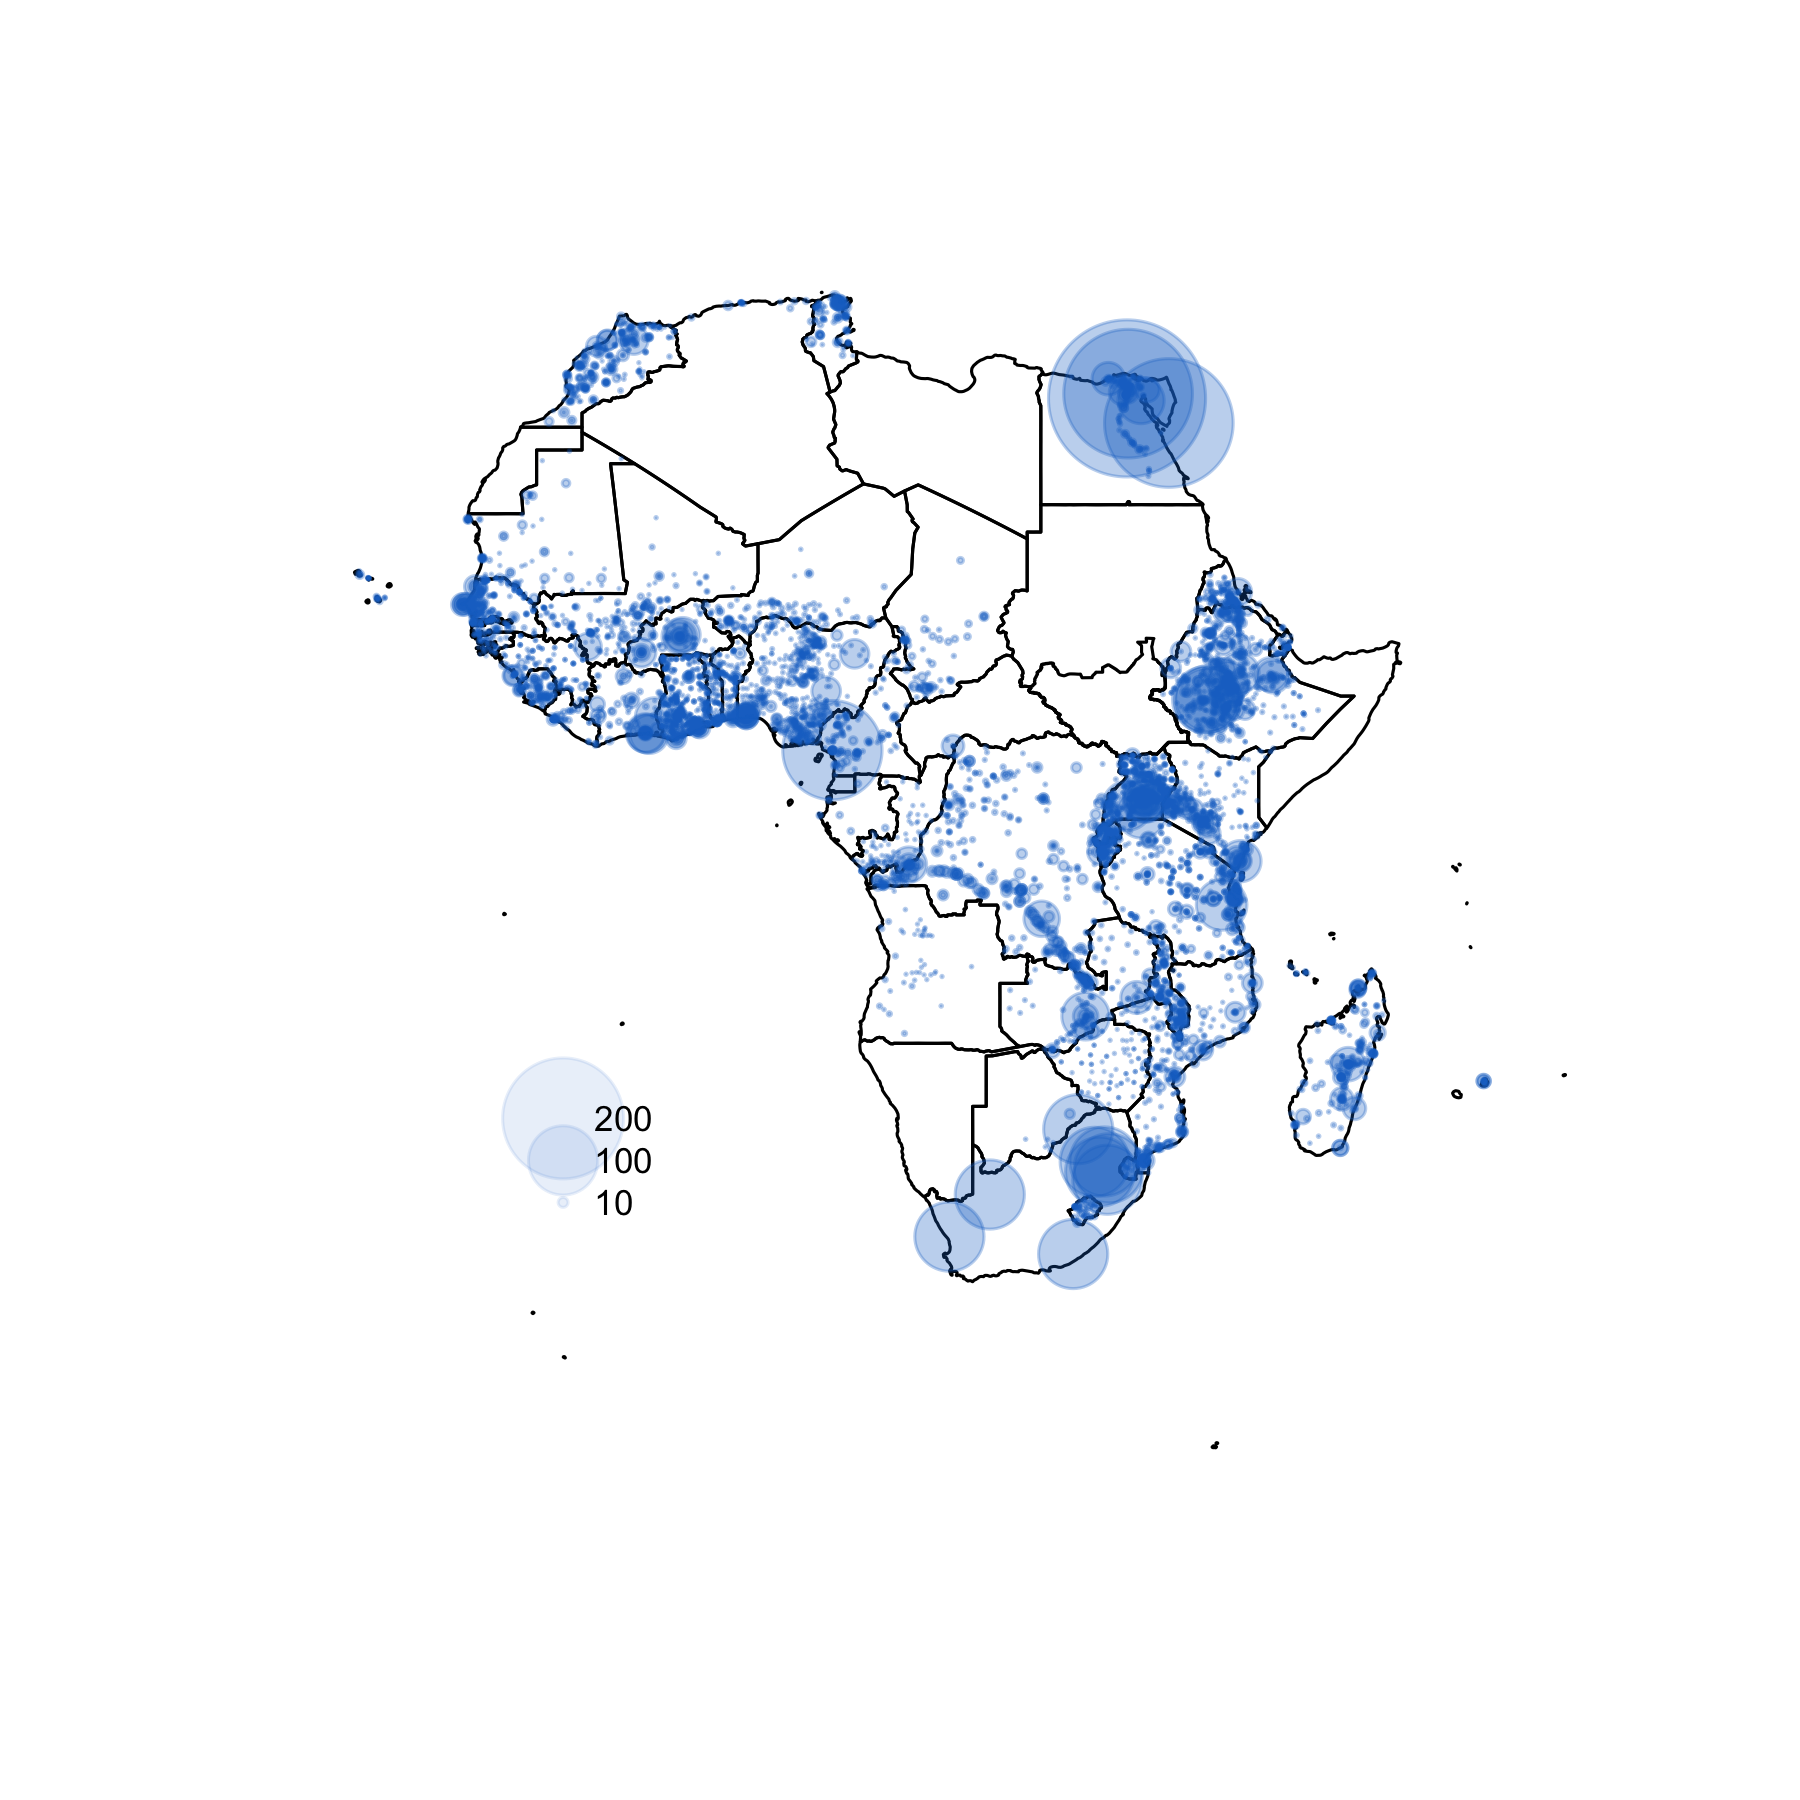
\includegraphics[width=\textwidth,trim={15cm 16cm 10cm 8cm},clip]{/Users/Tilmanski/Documents/UNI/MPhil/Second Year/Thesis_Git/Analysis/output/other_maps/aid_wb.png}
\caption{World Bank Aid}
\label{fig:WB_aid_map}
\end{subfigure}
\begin{subfigure}[c]{0.48\textwidth}
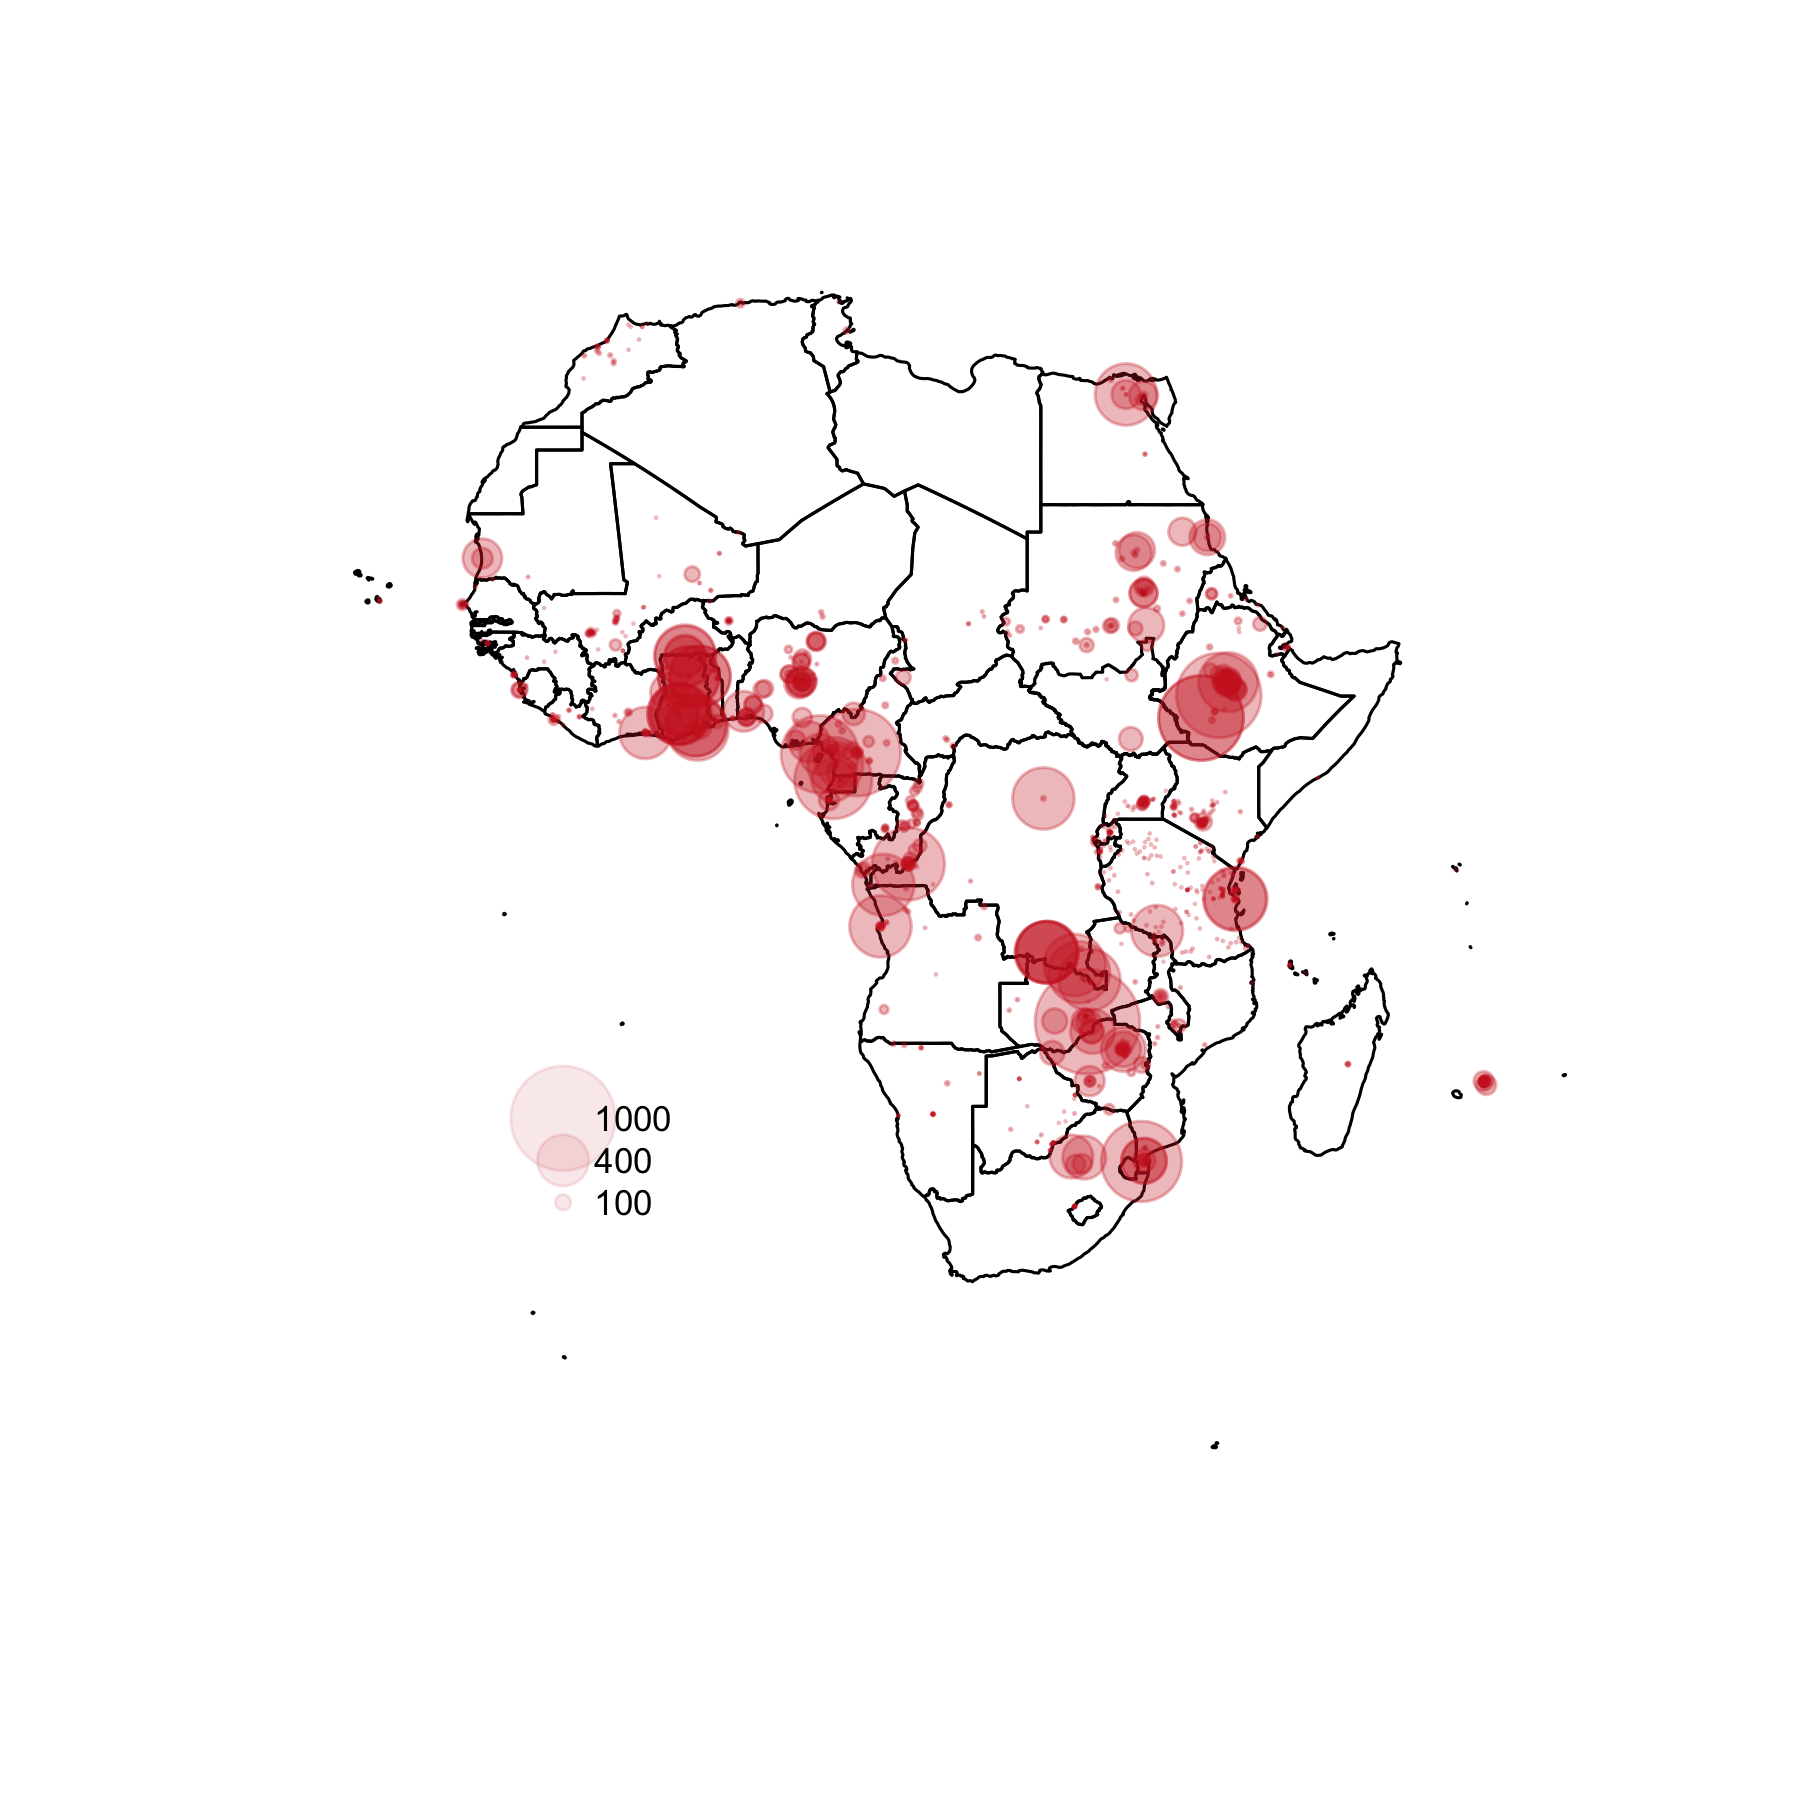
\includegraphics[width=\textwidth,trim={15cm 16cm 10cm 8cm},clip]{/Users/Tilmanski/Documents/UNI/MPhil/Second Year/Thesis_Git/Analysis/output/other_maps/aid_China.png}
\caption{Chinese Aid}
\label{fig:China_aid_map}
\end{subfigure}

\label{fig:Aid_maps}
\end{figure}
\end{frame}

\begin{frame}
\frametitle{Does Aid go into the right locations?}
\begin{table}[t] \centering
  \label{tab:RailKM_zeta}
  \resizebox{\textwidth}{!}{

  \begin{tabular}{@{\extracolsep{5pt}}lcccccccc}
  \\[-1.8ex]\hline
  \hline \\[-1.8ex]
   & \multicolumn{8}{c}{\textit{Dependent variable: Local Infrastructure Discrimination Index $\Lambda$}} \\
  \cline{2-9}
  \\[-1.8ex] & (1) & (2) & (3) & (4) & (5) & (6) & (7) & (8)\\
  \hline \\[-1.8ex]
  \multicolumn{9}{l}{\textit{Panel A: Worldbank Projects}} \\
  \\[-1.8ex]
  Total disbursements & $-$0.0003$^{***}$ & $-$0.0004$^{***}$ &  &  &  &  &  &  \\
  \hspace*{3mm} in million 2011 US dollars & (0.0001) & (0.0001) &  &  &  &  &  &  \\
   & & & & & & & & \\
  Transport-sector disbursements &  &  & $-$0.001$^{***}$ & $-$0.001$^{***}$ &  &  &  &  \\
   \hspace*{3mm} in million 2011 US dollars &  &  & (0.0002) & (0.0002) &  &  &  &  \\
   & & & & & & & & \\
  Number of projects &  &  &  &  & $-$0.002$^{***}$ & $-$0.003$^{***}$ &  &  \\
   &  &  &  &  & (0.0004) & (0.0004) &  &  \\
   & & & & & & & & \\
  Number of transport projects  &  &  &  &  &  &  & $-$0.003$^{***}$ & $-$0.004$^{***}$ \\
   &  &  &  &  &  &  & (0.001) & (0.001) \\
   & & & & & & & & \\
\\[-1.8ex]
 Country FE & Yes & Yes & Yes & Yes & Yes & Yes & Yes & Yes \\
 Geographic controls & Yes & Yes & Yes & Yes & Yes & Yes & Yes & Yes \\
 Simulation controls &  & Yes &  & Yes &  & Yes &  & Yes \\
 Observations & 10,158 & 10,158 & 10,158 & 10,158 & 10,158 & 10,158 & 10,158 & 10,158 \\
 R$^{2}$ & 0.125 & 0.128 & 0.125 & 0.127 & 0.127 & 0.131 & 0.126 & 0.129 \\
    \hline

% \multicolumn{9}{l}{\textit{Panel B: Chinese Development Projects}} \\
% \\[-1.8ex]
% Total commitments & $-$0.0001$^{***}$ & $-$0.0001$^{***}$ &  &  &  &  &  &  \\
%  \hspace*{3mm} in million 2011 US dollars & (0.00004) & (0.00004) &  &  &  &  &  &  \\
%  & & & & & & & & \\
% Transport-sector commitments &  &  & $-$0.0003$^{**}$ & $-$0.0003$^{**}$ &  &  &  &  \\
%  \hspace*{3mm} in million 2011 US dollars &  &  & (0.0001) & (0.0001) &  &  &  &  \\
%  & & & & & & & & \\
% Number of projects &  &  &  &  & $-$0.003$^{***}$ & $-$0.004$^{***}$ &  &  \\
%  &  &  &  &  & (0.001) & (0.001) &  &  \\
%  & & & & & & & & \\
% Number of transport projects &  &  &  &  &  &  & $-$0.013$^{***}$ & $-$0.014$^{***}$ \\
%  &  &  &  &  &  &  & (0.004) & (0.005) \\
%  & & & & & & & & \\
%  \\[-1.8ex]
% Country FE & Yes & Yes & Yes & Yes & Yes & Yes & Yes & Yes \\
% Geographic controls & Yes & Yes & Yes & Yes & Yes & Yes & Yes & Yes \\
% Simulation controls &  & Yes &  & Yes &  & Yes &  & Yes \\
% Observations & 10,158 & 10,158 & 10,158 & 10,158 & 10,158 & 10,158 & 10,158 & 10,158 \\
% R$^{2}$ & 0.123 & 0.125 & 0.123 & 0.125 & 0.124 & 0.126 & 0.123 & 0.125 \\
%  \hline
 \hline \\[-1.8ex]
 \textit{Note:}  & \multicolumn{8}{r}{$^{*}$p$<$0.1; $^{**}$p$<$0.05; $^{***}$p$<$0.01} \\
 \end{tabular}

}

\end{table}
\end{frame}



\begin{frame}
  \frametitle{Concerns}
  \begin{itemize}
    \item Identification
    \item Non-linearity of model
    \item ...
  \end{itemize}
\end{frame}


\begin{frame}
\label{backup:planners_problem}
  \frametitle{Backup: full planner's problem}
\fontsize{10}{7.2}\selectfont
  \begin{subequations}
  \begin{alignat*}{3}
  &\!\max_{\substack{\big\{C_{i}^{n}, \{Q_{i,k}^{n}\}_{k\in N(i)}\big\}_{n}, \\ c_{i}, \big\{I_{i,k}\big\}_{k\in N(i)}}}        &\qquad &  \sum_{i}^{} L_{i}u(c_{i}) \qquad &\\
  &\text{subject to} &\qquad & L_{i}c_{i} \leq \bigg( \sum_{n=1}^{N} (C_{i}^{n})^{\frac{\sigma-1}{\sigma}}\bigg)^{\frac{\sigma}{\sigma-1}} \qquad& \text{\textsc{\footnotesize \textbf{}}} \\
  &                  &\qquad & C_{i}^{n} + \sum_{k\in N(i)}^{}Q_{i,k}^{n}(1+\tau_{i,k}^{n}(Q_{i,k}^{n}, I_{i,k})) \leq Y_{i}^{n} + \sum_{j\in N(i)}^{}Q_{j,i}^{n} \qquad& \text{\textsc{\footnotesize \textbf{}}} \\
  &                  &\qquad & \sum_{i}^{}\sum_{k\in N(i)}^{}\delta^{i}_{i,k}I_{i,k} \leq K \qquad& \text{\textsc{\footnotesize \textbf{}}} \\
  &                  &\qquad & I_{i,k} = I_{k,i} \text{ for all } i\in \mathcal{I}, k\in N(i) \qquad& \text{\textsc{\footnotesize \textbf{}}} \\
  &                  &\qquad & C_{i}^{n}, c_{i}, Q_{i,k}^{n} \geq 0 \text{ for all } i \in \mathcal{I},n \in \mathcal{N},k\in N(i). \qquad& \text{\textsc{\footnotesize \textbf{}}}
  \end{alignat*}
  \end{subequations}
\hyperlink{trade_model}{\beamerbutton{Back}}
\end{frame}



\end{document}
